\chapter{فرایندهای تصادفی}
\label{ch2}
در فصل قبل به معرفی و بررسی متغیرهای تصادفی پرداختیم. در این فصل قصد داریم یک گام به جلو برداریم و به بررسی فرایندهای تصادفی\LTRfootnote{Stochastic process} بپردازیم. از فصل قبل می‌دانیم که $x$ یک متغیر تصادفی با توزیع احتمال $P(x)$ است.
فرایند تصادفی به دنباله‌ای از متغیرهای تصادفی گفته می‌شود مانند $x_{t_1}, x_{t_2}, \dotsc, x_{t_n}, \dotsc$ که پایین‌نویس‌های $\left\{ t_{i} \right\}$ می‌توانند نشان دهنده زمان باشند. اما در حالت کلی مجموعه‌ای  گسسته یا پیوسته است و لزوما معنای زمان نمی‌دهد. در ادامه مطلب از $\left\{ t_{i} \right\}$ به عنوان زمان استفاده خواهد شد اما محاسبات انجام شده در حالت کلی نیز درست است.
در هر نقطه زمانی $t_i$ (در حالت پیوسته از $t$ بدون پایین‌نویس استفاده خواهیم کرد) توزیع احتمال می‌تواند با زمان‌های دیگر متفاوت باشد. این وابستگی زمانی را می‌توان به شکل $P(x,t)$ برای توزیع احتمال و به شکل $p(x,t)$ برای چگالی احتمال نشان داد. اگر توزیع احتمال توأم یا چگالی احتمال توأم یک فرایند تصادفی یعنی $p(x_1,t_1;x_2,t_2;\dotsc x_n,t_n,\dotsc )$ را بدانیم، درواقع همه چیز را در مورد این فرایند تصادفی می‌دانیم چون می‌توانیم احتمال تمام مسیرهای ممکن برای فرایند تصادفی را محاسبه کنیم.\cite{2007cond.mat..1242G}
در حالت کلی برای یک فرایند تصادفی می‌توانیم بنویسیم.
\begin{equation}
  \begin{array}{l}
  p(x_n,t_n; x_{n-1},t_{n-1} \dotsc ;x_{0},t_0) \\ 
  \quad = p(x_{n},t_n \mid x_{n-1},t_{n-1} \dotsc ; x_{0},t_{0}) \dotsc p(x_{2},t_{2} \mid x_{1},t_{1};x_{0},t_{0}) p(x_{1},t_{1} \mid x_{0},t_{0}) p(x_0,t_0)
  \end{array}
  \label{n_point_joint}
\end{equation}
همان‌طور که از رابطه بالا مشخص است در اکثر موارد نمی‌توان این توزیع احتمال توأم را به دست آورد و در حالت کلی بررسی فرایندهای تصادفی به این  شکل کاری بسیار دشوار است. اما تا کنون حالت‌های خاص و مدل‌های مختلفی برای فرایندهای تصادفی ارائه شده است مانند فرایندهای مارکوف\LTRfootnote{Markov process}، یا مدل‌های پنهان مارکوف\LTRfootnote{Hidden Markov models} که هر کدام استفاده‌های مختلف و گسترده‌ای دارند. در شرایط تجربی علاقه‌مندیم که در صورت امکان مسائل خود را با مدل‌های موجود تخمین بزنیم بنابراین به ابزاری نیاز داریم تا بتوانیم امکان تخمین زدن مسائل با مدل‌های تصادفی را بررسی کنیم.

یکی ویژگی‌های مهم فرایندهای تصادفی مانا بودن یا نبودن آن‌ها است. اگر توزیع $n$ نقطه‌ای یک فرایند تصادفی به ازای $n$های مختلف وابستگی به زمان نداشته باشد، یعنی:
\begin{equation}
    p\left(x_{t_{1}+\tau}, \ldots, x_{t_{n}+\tau}\right)=p\left(x_{t_{1}}, \ldots, x_{t_{n}}\right)
\end{equation}
توزیع احتمال در سمت راست و چپ رابطه بالا به اندازه $\tau$ اختلاف زمانی دارند. اگر رابطه بالا برای یک فرایند تصادفی برقرار باشد آن فرایند مانا\LTRfootnote{Stationary} است. حالت‌های ضعیف‌تری برای مانا بودن یک فرایند وجود دارد مثلاً اگر میانگین و واریانس یک فرایند در زمان تغییر نکند به آن، فرایند مانای ضعیف گفته می‌شود.\cite{2007cond.mat..1242G}

\section{ولگشت تصادفی}
یکی از ساده‌ترین مثال‌ها برای فرایندهای تصادفی مسأله ولگشت تصادفی\LTRfootnote{Random walk} است. ذره‌ای را فرض کنید در هر زمان به شکل کاملاً تصادفی بر روی محور $x$ قدمی به سمت چپ یا راست بر می‌دارد.
در حالت کلی طول قدم‌ها می‌تواند متفاوت باشد اما حالتی را در نظر بگیرید که ذره در هر گام زمانی با احتمال $p$ یک قدم با طول یک به سمت راست برمی‌دارد و با احتمال $q$ یک قدم با طول یک به سمت چپ برمی‌دارد. بنابراین اگر قدم‌های این ذره را در گام زمانی $i$ام با $s_{i}$ نشان دهیم، بنابراین قدم‌های این ذره یک سری به شکل $s_{1}, s_{2}, \dotsc$ هستند که نشان دهنده یک فرایند تصادفی است که در هر زمان مقدار آن ۱+  یا ۱- است. اگر موقعیت مکانی این ذره در زمان $t_{i}$ با $x_{i}$ نشان دهیم، می‌توانیم آن را به صورت زیر محاسبه کنیم.
\begin{figure}[H]
  \centering
  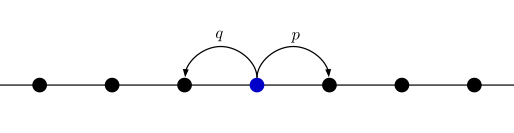
\includegraphics[scale=1]{images/simple_rw.png}
  \caption{ولگشت تصادفی ساده که با احتمال $p$ قدمی به سمت راست و با احتمال $q$ قدمی به سمت چپ برمی‌دارد.}
\end{figure}
\FloatBarrier
$$
  x_{n}=\sum_{i=1}^{n} s_{i}
$$
مسأله ولگشت تصادفی ساده را می‌توان در دو بعد و ابعاد بالاتر نیز بررسی کرد. در حالت کلی هیچ محدودیتی روی طول قدم‌ها وجود ندارد، مثلاً می‌توان حالتی را بررسی کرد طول قدم‌ها در هر زمان از یک توزیع گاوسی به شکل \ref{normal_dist} پیروی کند. در این شرایط انحراف معیار توزیع مکان این ولگشت تصادفی به شکل $\sigma_x \left( t \right) = \sqrt{t}$ تغییر می‌کند که نشان دهنده مانا نبودن این فرایند تصادفی است. در شکل زیر مکان چند نمونه مستقل از ولگشت تصادفی با قدم‌های گاوسی کشیده شده است، منحنی سیاه رنگ نشان دهنده انحراف از معیار $\sigma_x \left( t \right)$ است.
\begin{figure}[H]
  \centering
  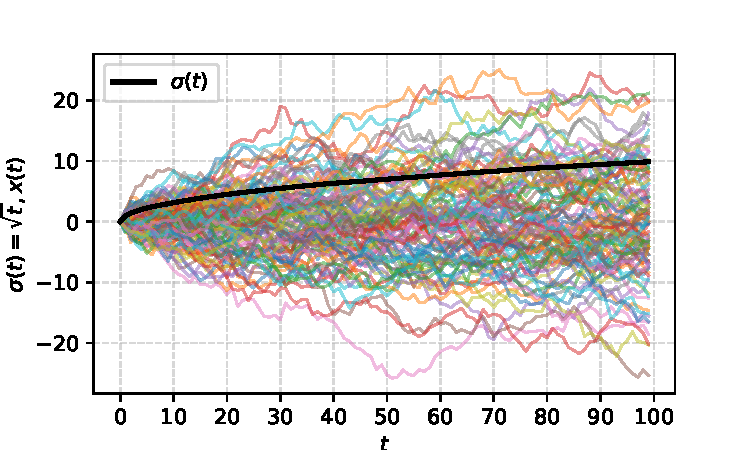
\includegraphics[width=0.9\textwidth]{images/normal_rw.pdf}
  \caption{چند نمونه مستقل از فرایند ولگشت تصادفی که قدم‌هایی با توزیع گاوسی برمی‌دارد.}
\end{figure}
\FloatBarrier

\section{فرایندهای مارکوف}
\label{sec:markov}

همان‌طور که گفته شد در صورتی که توزیع احتمال توأم $n$ نقطه‌ای  یک فرایند تصادفی را داشته باشیم، همه اطلاعات ممکن برای یک فرایند تصادفی تا زمان $t_n$ را می‌توانیم از روی توزیع احتمال توأم به دست آوریم. در حالتی که توزیع احتمال فرایند تصادفی در هر زمان به زمان‌های قبل از خودش وابستگی نداشته باشد و مستقل رفتار کند، توزیع احتمال توأم $n$ نقطه‌ای از ضرب احتمال متغیر تصادفی در زمان‌های مختلف به دست می‌آید. یعنی:
\begin{equation}
  p(x_n,t_n; x_{n-1},t_{n-1} \dotsc ;x_{0},t_0)  = p(x_{n}, t_{n}) p(x_{n-1}, t_{n-1}) \dotsc p(x_0,t_0)
  \label{n_point_joint}
\end{equation}
به فرایندی که از رابطه بالا پیروی کند فرایند تصادفی مستقل گفته می‌شود. کاربرد این‌گونه فرایندها بسیار محدود است، بنابراین به مدل‌های تصادفی بهتری نیاز داریم.
یکی از پرکاربرد ترین نوع فرایندهای تصادفی، فرایندهای مارکوف هستند. ایده اصلی فرایندهای مارکوف این است که حالت آینده یک فرایند تصادفی فقط به حالت کنونی فرایند وابسته است و از گام‌های زمانی قبل مستقل است پس می‌توان نتیجه گرفت که  توزیع احتمال این نوع فرایندها در هر زمان فقط به زمان قبلی وابسته است، یعنی:
\begin{equation}
  p(x_n,t_n \mid x_{n-1},t_{n-1} \dotsc ;x_{0},t_0) = p(x_n,t_n \mid x_{n-1},t_{n-1})
  \label{markov_def}
\end{equation}
 که رابطه بالا به ازای همه $n$ها برقرار است. بنابراین می‌توان توزیع احتمال توأم $n$ نقطه‌ای را به صورت زیر به دست آورد 
 \begin{equation}
  \begin{array}{l}
    p(x_n,t_n; x_{n-1},t_{n-1} \dotsc ;x_{0},t_0)\\ \qquad = p(x_{n},t_n\mid x_{n-1},t_{n-1}) \dotsc p(x_{2},t_{2} \mid x_{1},t_{1}) p(x_{1},t_{1} \mid x_{0},t_{0}) p(x_0,t_0)
    \label{markov}
  \end{array}
\end{equation}
به احتمال‌های شرطی دو تایی در فرایندهای مارکوف، احتمال انتقال هم گفته می‌شود در شرایطی که این احتمال به زمان وابستگی نداشته باشد و فقط به اختلاف زمانی وابسته باشد به این فرایند، فرایند همگن\LTRfootnote{Homogenous Markov chain} گفته می‌شود. 
به عنوان مثالی از فرایندهای مارکوف همگن فرض کنید اگر امروز هوا آفتابی یا بارانی باشد بر روی شرایط آب و هوای فردا تأثیر گذار باشد و مهم نباشد که در چو موقعی از سال قرار داریم. شکل زیر نمایشی از ماتریس انتقال برای این مثال است.
\begin{figure}[H]
  \centering
  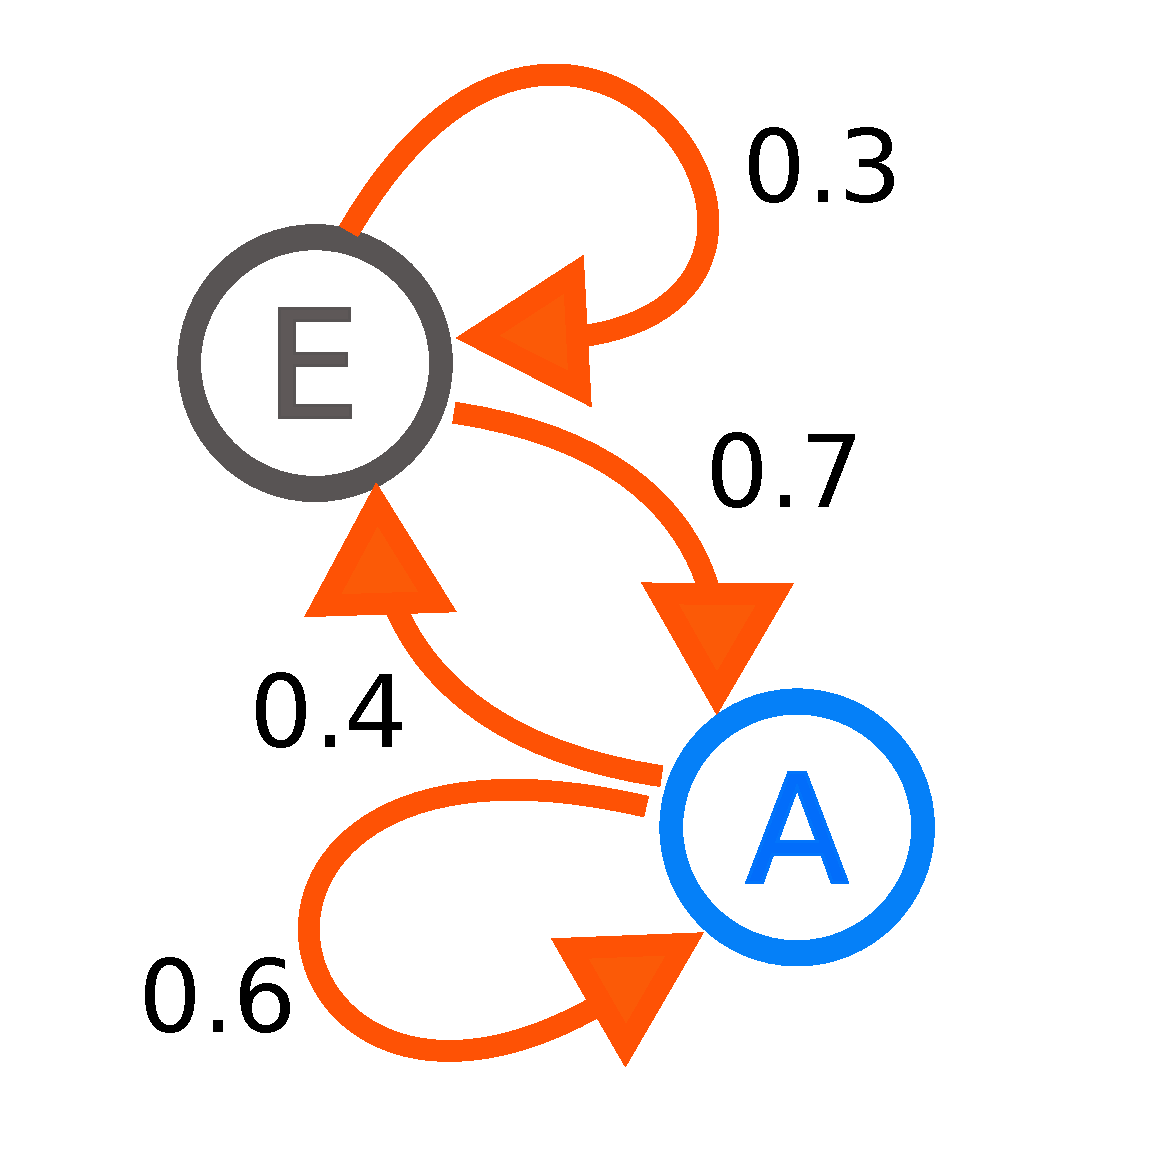
\includegraphics[width=0.4\textwidth]{images/weather_chain.pdf}
  \caption{زنجیره مارکوف} \label{fig:weather_chain}
  \par\medskip
\captionsetup{justification=centering}
\end{figure}
\FloatBarrier

اغلب به فرایندهای مارکوف با زمان گسسته و فضای نمونه شمارا، زنجیره مارکوف هم گفته می‌شود. در جدول زیر انواع فرایندهای مارکوف در شرایط مختلف آورده شده است، هرچند بر روی این تقسیم‌بندی و برخی اصطلاحات توافقی وجود ندارد. اما استفاده از نام زنجیره مارکوف برای فرایندهای با زمان و فضای نمونه گسسته رایج است.\cite{gagniuc_markov_2017}
\begin{table}[htb]
  \centering
  \caption{تقسیم‌بندی فرایندهای مارکوف}
  \begin{tabular}{|C{4cm}|C{4cm}|C{4cm}|}
    \hline
    \cellcolor[HTML]{C0C0C0} & فضای نمونه شمارا                               & فضای نمونه پیوسته                             \\ \hline
    زمان گسسته               & زنجیره مارکوف                                  & زنجیره مارکوف روی فضای نمونه قابل اندازه‌گیری \\ \hline
    زمان پیوسته              & فرایند مارکوف زمان‌پیوسته یا فرایند پرش مارکوف & دیگر فرایندهای تصادفی با خاصیت مارکوف         \\ \hline
    \end{tabular}
\end{table}
\FloatBarrier

از این پس تمام روابط برای فرایند مارکوف با فضای نمونه و زمان پیوسته نوشته خواهند شد اما در ادامه به بررسی چند ویژگی مهم می‌پردازیم که بیشتر برای زنجیره‌های مارکوف استفاده می‌شوند.

\subsection{حد مانای فرایندهای مارکوف}

برخی فرایندهای مارکوف پس از گذشت زمان کافی به حالتی مانا می‌رسند.
در این بخش به بررسی روشی برای یافتن حالت مانا فرایندهای مارکوف می‌پردازیم که بیشتر برای زنجیره‌های مارکوف کاربردی است.
با توجه به رابطه \ref{j_prob_cond} می‌توانیم بنویسیم.
$$
  p(x_{i+1},t_{i+1};x_{i}, t_{i}) = p(x_{i+1},t_{i+1} \mid x_{i}, t_{i}) p(x_{i},t_{i})
$$
که $x_i$ و $x_{i+1}$، متغیر تصادفی $x$ را در دو زمان متوالی $t_i$ و $t_{i+1}$ نشان می‌دهد. با استفاده از رابطه \ref{marginalization} و جمع زدن بر روی $x_i$ می‌توانیم توزیع احتمال $x_{i+1}$ را در زمان $t_{i+1}$ به دست آوریم.
\begin{equation}
  p(x_{i+1},t_{i+1}) = \int_{-\infty}^{+\infty} p(x_{i+1},t_{i+1} \mid x_{i}, t_{i}) p(x_{i},t_{i}) d x_{i}
  \label{transition_multip}
\end{equation}
رابطه بالا در‌واقع نشان دهنده ضرب ماتریس انتقال $\mathbf{p_{i+1,i}}$ در بردار توزیع احتمال $\mathbf{p_i}$ است.
$$
  \mathbf{p_{i+1}} = \mathbf{p_{i+1,i}} \times \mathbf{p_i}
$$
که حروف پررنگ نشان‌دهنده شکل ماتریسی و برداری است.
اگر $\mathbf{p_{i+2,i+1}}$ را در دو طرف رابطه بالا ضرب کنیم.
$$
  \mathbf{p_{i+2}} = \mathbf{p_{i+2,i+1}} \times \mathbf{p_{i+1,i}} \times \mathbf{p_i}
$$
در حالتی که فرایند همگن باشد یعنی $p(x_{i+2}, t_{i+2} \mid x_{i+1},t_{i+1})=p(x_{i+1},t_{i+1} \mid x_{i}, t_{i})$ باشد و ماتریس انتقال را نیز با $\mathbf{W}=\mathbf{p_{i+2,i+1}} = \mathbf{p_{i+1,i}}$ نشان دهیم خواهیم داشت.
$$
  \mathbf{p_{i+2}} = \mathbf{W}^{2} \times \mathbf{p_{i}}
$$
رابطه بالا یکی از نتیاج مهم برای فرایندهای مارکوف همگن است، اگر این کار را ادامه دهیم می‌توانیم احتمال انتقال برای $n$ گام زمانی را برای یک فرایند مارکوف همگن به دست آوریم. که به شکل زیر به دست می‌آید.
\begin{equation}
    \mathbf{p_{n}} = \mathbf{W}^{n} \times \mathbf{p_{0}}
    \label{nstep_transition}
\end{equation}
با فرض اینکه حالت مانای فرایند $x$ وجود دارد و $p_{s}(x)$ نشان دهنده توزیع احتمال $x$ در زمان $t_s$ باشد یعنی زمانی که فرایند به حالت مانای خود رسیده است، اگر ماتریس انتقال را در این احتمال ضرب کنیم، توزیع به دست آمده باید برابر $p_{s}(x)$ باشد.\cite{bremaud_markov_1999}
$$
\mathbf{p_{s}(x)} = \mathbf{W}^{n} \times \mathbf{p_{s}(x)}
$$
رابطه بالا در فیزیک به معادله ویژه برداری معروف است، با حل این معادله می‌توان $p_{s}(x)$ را به دست آورد.

\subsection{معادله چَپمَن-کولموگروف}

با توجه به رابطه \ref{marginalization} دیدیم که توزیع‌های احتمال توأم چگونه به هم مرتبط هستند اگر بخواهیم احتمال توأم دونقطه‌ای را از احتمال توأم سه نقطه‌ای به دست آوریم داریم:
$$
  p\left(x_{3}, t_{3} ; x_{1}, t_{1}\right)=\int_{-\infty}^{+\infty} p\left(x_{3}, t_{3}; x_{2}, t_{2}; x_{1}, t_{1}\right) d x_{2}
$$
 اگر $x$ یک فرایند مارکوف باشد بنابراین $p(x_{3}, t_{3} ; x_{2}, t_{2}; x_{1}, t_{1}) = p(x_{3}, t_{3} \mid x_{2}, t_{2}) p(x_{2}, t_{2} \mid x_{1}, t_{1}) p(x_{1}, t_{1})$ با جایگذاری در رابطه بالا داریم:
 \begin{equation}
  p\left(x_{3}, t_{3}; x_{1}, t_1\right)=\int_{-\infty}^{+\infty} p\left(x_{3}, t_3 \mid x_{2}, t_2\right) p\left(x_{2}, t_2 \mid x_{1}, t_1\right) p\left(x_{1}, t_1\right) d x_{2}
  \label{ck_equation}
\end{equation}
معادله بالا به معادله چپمن-کولموگروف\LTRfootnote{Chapman-Kolmogorov equation} معروف است و باید توجه شود که معادله بالا برای سه زمان متوالی $t_1$، $t_2$ و $t_3$ نوشته شده است. اگر دو طرف تساوی را به $p(x_{1}, t_1)$ تقسیم کنیم با توجه به رابطه احتمال شرطی و توأم \ref{cond_prob_j} به شکل دیگری از معادله چپمن-کولموگروف می‌رسیم.
\begin{equation}
  p\left(x_{3}, t_3 \mid x_{1}, t_1\right)=\int_{-\infty}^{+\infty} p\left(x_{3}, t_3 \mid x_{2}, t_2\right) p\left(x_{2}, t_2 \mid x_{1}, t_1\right) d x_{2}
  \label{ck_equation_cond}
\end{equation}
معادله چپمن-کولموگروف برای همه‌ی فرایندهای مارکوف برقرار است، اما هر فرایندی که معادله چپمن-کولموگروف برای آن برقرار باشد لزوماً مارکوف نیست. به عبارت دیگر برقرار بودن معادله چپمن-کولموگروف شرط لازم برای یک فرایند مارکوف است.

\subsection{فرایند وینر}

یک مثال پرکاربرد از فرایندهای مارکوف، فرایند وینر\LTRfootnote{Wiener process} است. فرایند وینر از بسیاری جهات مشابه یک ولگشت تصادفی با قدم‌های گاوسی است، با این تفاوت که توزیع قدم‌ در هر زمان به قدم قبلی وابسته است. احتمال انتقال فرایند وینر به شکل زیر است:
\begin{equation}
  p_{2}\left(x, t \mid x^{\prime}, t^{\prime}\right)=\frac{1}{\sqrt{2 \pi \tau}} e^{-\left(x-x^{\prime}\right)^{2} / 2 \tau}
\end{equation}
که $\tau = t - t^\prime$ است، بنابراین فرایند وینر یک فرایند مارکوف همگن است که احتمال انتقال آن فقط به $\tau$ وابسته است. توزیع احتمال این فرایند در هر زمان به شکل زیر است.
\begin{equation}
  p_{1}(x, t)=\frac{1}{\sqrt{2 \pi t}} e^{-x^{2} / 2 t}
  \end{equation}
فرایند وینر را در فیزیک می‌توان به عنوان فرایند پخش گرما یا حرکت براونی ذرات تعبیر کرد. نکته مهم در مورد فرایند وینر این است که این فرایند حد مانا ندارد.\cite{risken_fokker-planck_1984}

\subsection{معادله مادر}

برای فهمیدن رفتار یک فرایند مارکوف معادله چپمن-کولموگروف کمک زیادی نخواهد کرد اما می‌توان از معادله چپمن-کولموگروف به معادله‌ای سودمند به نام معادله مادر\LTRfootnote{Master equation} رسید. 
معادله مادر یک معادله دیفرانسیلی برای احتمال انتقال است که تغییرات احتمال انتقال بر حسب زمان را به دست می‌دهد. برای به دست آوردن این معادله باید رفتار احتمال انتقال را در اختلاف زمان‌های کوتاه یعنی $\Delta t \rightarrow 0$ مشخص کنیم. در معادله \ref{ck_equation_cond} به ازای $t_2 = t_1 = t$ به نتیجه بدیهی زیر می‌رسیم.
$$
\begin{array}{l}
  p\left(x_{3} , t_{3} \mid x_{1} , t_{1}\right) = \int_{-\infty}^{+\infty} p\left(x_{3} , t_{3} \mid x_{2} , t \right) p\left(x_{2} , t \mid x_{1} , t \right) d x_{2} \\
  \qquad \Rightarrow p\left(x_{2} , t \mid x_{1} , t \right) = \delta\left( x_2 - x_1 \right) 
\end{array}
$$
که تابع دلتا به دست آمده در‌واقع مرتبه صفرم از رفتار $p(x^\prime,t^\prime \mid x,t)$ در زمان‌های کوتاه است. با در نظر داشتن این نکته می‌توان رابطه زیر را برای رفتار احتمال انتقال در زمان‌های کوتاه به دست آورد.
\begin{equation}
  p\left(x_{2}, t+\Delta t \mid x_{1}, t\right)=\delta\left(x_{2}-x_{1}\right)\left[1-a^{(0)}\left(x_{1}, t\right) \Delta t\right]+w_{t}\left(x_{2} \mid x_{1}\right) \Delta t+O\left[(\Delta t)^{2}\right]
  \label{transition_zero_order}
\end{equation}
در رابطه بالا $w_{t}(x_2 \mid x_1)$ را به عنوان احتمال انتقال از $x_{1}$ به $x_{2}$ بر واحد زمان $t$ تعبیر می‌کنیم. بنابراین ضریب $1-a^{(0)}\left(x_{1}, t\right) \Delta t$ را باید احتمال اینکه هیچ انتقالی در مدت زمان $\Delta t$ صورت نگیرد تعبیر کرد یعنی احتمال اینکه در این مدت زمان  $x$ ثابت باشد. از نرمال بودن احتمال انتقال $p(x_2,t_2 \mid x_1,t_1)$ می‌توانیم بنویسیم.
$$
1=\int \mathrm{d} x_{2} P\left(x_{2}, t+\Delta t \mid x_{1}, t\right) \simeq 1-a^{(0)}\left(x_{1}, t\right) \Delta t+\int \mathrm{d} x_{2} w_{t}\left(x_{2} \mid x_{1}\right) \Delta t
$$
بنابراین داریم
\begin{equation}
  a^{(0)}\left(x_{1}, t\right)=\int \mathrm{d} x_{2} w_{t}\left(x_{2}  \mid  x_{1}\right)
  \label{cond_moment_zero}
\end{equation}
از رابطه بالا می‌بینیم که $a^{(0)}\left(x_{1}, t\right) \Delta t$ احتمال کل انتقال از $x_{1}$ در بازه $(t,t+\Delta t)$را نشان می‌دهد بنابراین $1 - a^{(0)}\left(x_{1}, t\right) \Delta t$ احتمال این است که هیچ انتقالی در این بازه اتفاق نیفتد.

حالا می‌توانیم با استفاده از معادله چپمن-کولموگروف \ref{ck_equation_cond} معادله دیفرانسیلی برای احتمال انتقال به دست آوریم. با جایگذاری رابطه \ref{transition_zero_order} در معادله چپمن-کولموگروف \ref{ck_equation_cond} به ازای $t_{3} = t_{2} + \Delta t$ داریم:

$$
\begin{aligned} p\left(x_{3}, t_{2}+\Delta t  \mid  x_{1}, t_{1}\right)=& \int \mathrm{d} x_{2} \overbrace{p\left(x_{3}, t_{2}+\Delta t \mid x_{2}, t_{2}\right)}^{\hidewidth \delta\left(x_{3}-x_{2}\right)\left[1-a^{(0)}\left(x_{2}, t_{2}\right) \Delta t\right]+w_{t_{2}}\left(x_{3}  \mid  x_{2}\right) \Delta t \hidewidth } p\left( x_{2}, t_{2} \mid x_{1} , t_{1} \right)\\ \simeq &\left[1-a^{(0)}\left(x_{3}, t_{2}\right) \Delta t\right] p\left(x_{3}, t_{2}  \mid  x_{1}, t_{1}\right) \\ &+\Delta t \int \mathrm{d} x_{2} w_{t_{2}}\left(x_{3}  \mid  x_{2}\right) p\left(x_{2}, t_{2}  \mid  x_{1}, t_{1}\right) \end{aligned}
$$
 سپس  $a^{(0)}\left(x_{3}, t_{2}\right)$ را با استفاده از \ref{cond_moment_zero} بر حسب $w_{t_{2}}(x_{2} \mid x_{3})$ می‌نویسیم. بنابراین رابطه بالا را به شکل زیر می‌نویسیم.
$$
\begin{aligned} \frac{1}{\Delta t}\left[p\left(x_{3}, t_{2}\right.\right.&\left.\left.+\Delta t \mid x_{1}, t_{1}\right)-p\left(x_{3}, t_{2} \mid x_{1}, t_{1}\right)\right] \\ & \simeq \int \mathrm{d} x_{2}\left[w_{t_{2}}\left(x_{3} \mid x_{2}\right) p\left(x_{2}, t_{2} \mid x_{1}, t_{1}\right)-w_{t_{2}}\left(x_{2} \mid x_{3}\right) p\left(x_{3}, t_{2} \mid x_{1}, t_{1}\right)\right] \end{aligned}
$$
نشان گذاری  را با تبدیل $x_{1}$ و $t_{1}$ به $x_{0}$ و $t_{0}$، $x_{2}$ و $t_{2}$ را به $x^\prime$ و $t^\prime$   و در نهایت $x_{3}$ را به $x$ تغییر می‌دهیم. بنابراین در حد $\Delta t \rightarrow 0$ می‌توانیم معادله مادر را به شکل زیر به دست آوریم.
\begin{equation}
  \frac{\partial}{\partial t} p\left(x, t \mid x_{0}, t_{0}\right)=\int \mathrm{d} x^{\prime}\left[w_{t}\left(x | x^{\prime}\right) p\left(x^{\prime}, t \mid x_{0}, t_{0}\right)-w_{t}\left(x^{\prime} \mid x\right) p\left(x, t \mid x_{0}, t_{0}\right)\right]
  \label{master_equation_transition}
\end{equation}
که یک معادله انتگرال – دیفرانسیل است. معادلات انتگرال – دیفرانسیل معادلاتی هستند که شامل انتگرال و مشتق یک تابع هستند.

معادله مادر یک شکل دیفرانسیلی از معادله چپمن-کولموگروف است. بنابراین نمی‌توان با آن توزیع احتمال $p\left( x, t \right)$ را حساب کرد و برای محاسبه احتمال انتقال $p\left( x,t \mid x_{0},t_{0} \right)$ کاربرد دارد. اما می‌توان نشان داد که با در نظر گرفتن شرایط اولیه می‌توان معادله‌ای برای توزیع احتمال با استفاده از معادله مادر به شکل زیر به دست آورد.\cite{2007cond.mat..1242G}
\begin{equation}
  \frac{\partial p(x, t)}{\partial t}=\int \mathrm{d} x^{\prime}\left[w\left(x \mid x^{\prime}\right) p\left(x^{\prime}, t\right)-w\left(x^{\prime} \mid x\right) p(x, t)\right]
  \label{master_equation}
\end{equation}
از شکل معادله مادر می‌بینیم که این معادله در‌واقع یک معادله توازن برای احتمال حالت‌های (مقادیر) ممکن $x$ است.

\subsection{بسط کرامرز-مویال و معادله فوکر-پلانک}

بسط کرامرز-مویال\LTRfootnote{Kramers–Moyal expansion} معادله مادر را از یک معادله انتگرال – دیفرانسیل به یک معادله دیفرانسیل با مرتبه بی‌نهایت تبدیل می‌کند. بنابراین استفاده از این بسط از معادله مادر آسان‌تر نیست اما تحت شرایطی ممکن است که بتوان با تعداد محدودی از جملات بسط معادله را حل کرد.\cite{kramers_brownian_1940}

در ابتدا با یک تغییر متغیر احتمال انتقال $w$ را به تابعی بر حسب $r$ که $r=x^\prime - x$ تبدیل می‌کنیم. یعنی احتمال انتقال تابعی است از میزان جابه‌جایی $r$ و نقطه شروع $x^\prime$، بنابراین داریم:
\begin{equation}
  w\left( x \mid x^{\prime} \right) = w\left(x^{\prime} ; r\right), \quad r=x-x^{\prime}
  \label{transition_cfv}
\end{equation}
بنابراین معادله مادر \ref{master_equation} را می‌توان به شکل زیر نوشت.
\begin{equation}
  \frac{\partial p(x, t)}{\partial t}=\int w(x-r ; r) p(x-r, t) \mathrm{d} r - p(x, t) \int w(x ;-r) \mathrm{d} r
  \label{master_eq_1}
\end{equation}
 که تغییر علامت مربوط به تغییر متغیر $x^\prime \rightarrow r = x - x^\prime$ در کران‌های انتگرال به این شکل تأثیر گذاشته است که
$$
  \int_{-\infty}^{\infty} \mathrm{d} x^{\prime} f\left(x^{\prime}\right)=-\int_{x+\infty}^{x-\infty} \mathrm{d} r f(x-r)=-\int_{\infty}^{-\infty} \mathrm{d} r f(x-r)=\int_{-\infty}^{\infty} \mathrm{d} r f(x-r)
$$
با فرض اینکه تغییرات $x$ به شکل پرش‌های کوچک اتفاق می‌افتد بنابراین $w(x^\prime;r)$ یک تابع تیز از $r$ است اما تغییرات آن با $x^\prime$ به اندازه کافی آرام است. فرض دیگری که می‌کنیم این است که $p(x,t)$ نیز به آرامی با $x$ تغییر می‌کند. حال می‌توانیم تغییر $x$ به $x-r$ را با بسط تیلور بررسی کنیم بنابراین جمله اول سمت راست رابطه \ref{master_eq_1} را بسط تیلور می‌دهیم.
$$
\begin{aligned} \frac{\partial p(x, t)}{\partial t}=& \int w(x ; r) p(x, t) \mathrm{d} r+\sum_{m=1}^{\infty} \frac{(-1)^{m}}{m !} \int r^{m} \frac{\partial^{m}}{\partial x^{m}}[w(x ; r) p(x, t)] \mathrm{d} r  \\ &-p(x, t) \int w(x ;-r) \mathrm{d} r \\=& \sum_{m=1}^{\infty} \frac{(-1)^{m}}{m !} \frac{\partial^{m}}{\partial x^{m}}\left\{\left[\int r^{m} w(x ; r) \mathrm{d} r \right] p(x, t)\right\} \end{aligned}
$$
که جمله اول و سوم در رابطه بالا با یکدیگر ساده شده‌اند بنابراین داریم.
در انتها ضرایب بسط به شکل زیر تعریف می‌کنیم.
\begin{equation}
  a^{(m)}(x, t)=\int r^{m} w(x ; r) \mathrm{d} r
  \label{jump_moments}
\end{equation}
بنابراین بسط کرامرز-مویال معادله مادر به شکل زیر به دست می‌آید. 
\begin{equation}
  \frac{\partial p(x, t)}{\partial t}=\sum_{m=1}^{\infty} \frac{(-1)^{m}}{m !} \frac{\partial^{m}}{\partial x^{m}}\left[a^{(m)}(x, t) p(x, t)\right]
  \label{kramers_moyal}
\end{equation}
بسط کرامرز-مویال هیچ تفاوتی با معادله مادر ندارد پس استفاده از این بسط به اندازه معادله مادر مشکل است. اما همان‌طور که گفته شد ممکن است تحت شرایطی بتوان از جملات مرتبه بالا بسط کرامز مویال صرف نظر کرد. مثلاً در شرایطی که به ازای $m > 2$ ضرایب $a^{m}(x,t)$ خیلی کوچک باشند و بتوان از آن‌ها صرف نظر کرد، بسط کرامرز-مویال به شکل زیر تبدیل می‌شود.
\begin{equation}
  \frac{\partial p(x, t)}{\partial t}=-\frac{\partial}{\partial x}\left[a^{(1)}(x, t) p(x, t)\right]+\frac{1}{2} \frac{\partial^{2}}{\partial x^{2}}\left[a^{(2)}(x, t) p(x, t)\right]
  \label{fokker_plank}
\end{equation}
به معادله بالا، معادله فوکر-پلانک\LTRfootnote{Fokker–Planck equation} گفته می‌شود. به جمله اول این معادله جمله رانش و به جمله دوم آن جمله پخش گفته می‌شود، همچنین به ضرایب $a^{1}(x,t)$ و $a^{2}(x,t)$ ضریب رانش و ضریب پخش گفته می‌شود. یادآوری این نکته لازم است که معادله فوکر-پلانک به عنوان حالت خاصی از بسط کرامرز-مویال از معادله مادر به دست می‌آید، بنابراین این معادله نیز رفتار احتمال انتقال را در زمان نشان می‌دهد اما همان‌طور که گفته شد با در نظر گرفتن شرایط اولیه می‌توان رفتار توزیع احتمال را همان‌طور که در \ref{fokker_plank} نوشته شده است نیز به دست آورد.\cite{moyal_stochastic_1949}

\subsection{ممان‌های شرطی}

احتمال انتقال بر واحد زمان $w(x^\prime \mid x)$ در تعریف ممان‌های شرطی \ref{jump_moments} استفاده شده است. بنابراین مجبوریم برای محاسبه $a^{m}(x.t)$ از رابطه \ref{transition_zero_order} که رابطه بین $w(x^\prime \mid x)$ و احتمال انتقال برای اختلاف زمان‌های کوچک است، استفاده کنیم.
در رابطه \ref{transition_cfv} دیدیم که $w(x^\prime ; r) = w(x \mid x^\prime)$ و $x = x^\prime + r$ بر همین اساس می‌توانیم بنویسیم:
$$
w(x ; r)=w\left(x^{\prime} \mid x\right), \quad x^{\prime}=x+r
$$
با جایگذاری این عبارت در معادله \ref{jump_moments} می‌توان نوشت.
\begin{equation}
  a^{(m)}(x, t)=\int \mathrm{d} x^{\prime}\left(x^{\prime}-x\right)^{m} w\left(x^{\prime} \mid x\right)
\end{equation}
به منظور اینکه رابطه‌ای برای ضرایب به دست بیاوریم کمیت زیر را معرفی می‌کنیم.
\begin{equation}
  \mathcal{A}^{(m)}(x ; \tau, t)=\int \mathrm{d} x^{\prime}\left(x^{\prime}-x\right)^{m} p\left(x^{\prime}, t+\tau \mid x, t\right)
\end{equation}
که در‌واقع میانگین $[X(t + \tau) - X(t)]^{m}$ به ازای $X(t) = x$ است و به آن ممان شرطی می‌گویند. سپس با استفاده از احتمال انتقال برای زمان‌های کوتاه \ref{transition_zero_order} می‌توانیم بنویسیم

$$
\begin{aligned} \mathcal{A}^{(m)}(x ; \tau, t) &=\int \mathrm{d} x^{\prime}\left(x^{\prime}-x\right)^{m}\left\{\delta\left(x^{\prime}-x\right)\left[1-a^{(0)}(x, t) \tau\right]+w\left(x^{\prime} \mid x\right) \tau+\mathcal{O}\left(\tau^{2}\right)\right\} \\ &=\tau \int \mathrm{d} x^{\prime}\left(x^{\prime}-x\right)^{m} w\left(x^{\prime} \mid x\right)+\mathcal{O}\left(\tau^{2}\right) \\ &=a^{(m)}(x, t) \tau+\mathcal{O}\left(\tau^{2}\right), \quad(m \geq 1) \end{aligned}
$$
که اولین جمله انتگرال به دلیل وجود تابع دلتای دیراک از بین می‌رود. بنابراین می‌توان ضرایب بسط را از مشتق ممان‌های شرطی به شکل زیر به دست آورد
\begin{equation}
a^{(m)}(x, t)=\left.\frac{\partial}{\partial \tau} \mathcal{A}^{(m)}(x ; \tau, t)\right|_{\tau=0}
\label{cond_moment_km}
\end{equation}
در انتها با نوشتن $\mathcal{A}$ به شکل زیر:
$$
\mathcal{A}^{(m)}(x ; \Delta t, t)=\int \mathrm{d} x^{\prime}\left(x^{\prime}-x\right)^{m} p\left(x^{\prime}, t+\Delta t  \mid  x, t\right)=\left.\left\langle[X(t+\Delta t)-X(t)]^{m}\right\rangle\right|_{X(t)=x}
$$
می‌توانیم ضرایب بسط را با استفاده از رابطه زیر به دست آوریم.
\begin{equation}
a^{(m)}(x, t)=\left.\lim _{\Delta t \rightarrow 0} \frac{1}{\Delta t}\left\langle[X(t+\Delta t)-X(t)]^{m}\right\rangle\right|_{X(t)=x}
\label{exp_coef}
\end{equation}

\subsection{قضیه پاوولا}
همان‌طور که دیدیم بسط کرامرز-مویال دارای تعداد نامتناهی جمله است که در حالت کلی حل این بسط را نسبت به معادله مادر ساده‌تر نمی‌کند، اما اگر بتوان تعدادی از جملات را نگه داشت و از بقیه آن‌ها صرف نظر کرد حل بسط کرامرز-مویال بسیار ساده‌تر از معادله مادر خواهد بود. برای اینکه بتوانیم از این جملات صرف نظر کنیم، ممان‌های متعلق به این جملات باید صفر باشند. اما بررسی کردن تعداد نامتناهی ممان به اندازه حل بسط کرامرز-مویال کار دشواری است. با روشی که قضیه پاوولا\LTRfootnote{Pawula theorem} معرفی می‌کند می‌توانیم از صفر بودن ممان‌ها، بدون بررسی تک‌تک آن‌ها مطمئن شویم. 
بدین منظور باید از حالت کلی نامساوی شوارتز استفاده کنیم که به شکل زیر است.
\begin{equation}
  [f(x) g(x) P(x) \mathrm{d} x]^{2} \leq \int f^{2}(x) P(x) \mathrm{d} x \int g^{2}(x) P(x) \mathrm{d} x
\end{equation}
در نامساوی بالا $P(x)$ یک تابع مثبت است و توابع $f(x)$ و $g(x)$ توابع دلخواهی هستند.
$$
\begin{array}{l}{f(x)=\left(x-x^{\prime}\right)^{n} ; \quad g(x)=\left(x-x^{\prime}\right)^{n+m}} \\ {P(x)=P\left(x, t+\tau | x^{\prime}, t^{\prime}\right)}\end{array}
$$
به ازای توابع به شکل بالا نامساوی شوارتز به عبارت زیر که بین ممان‌های شرطی است تبدیل می‌شود.\cite{risken_fokker-planck_1984}
\begin{equation}
  \mathcal{A}_{2 n+m}^{2} \leq \mathcal{A}_{2 n} \cdot \mathcal{A}_{2 n+2 m}
  \label{inequality_moments}
\end{equation}
برای $n=0$ داریم $\mathcal{A}_{m} \leq \mathcal{A}_{2m}$  که این رابطه به وضوح برای $m = 0$ برقرار است. از این رابطه هیچ محدودیتی برای ضرایب بسط $a^{(m)}(x, t)$ به دست نمی‌آید. به ازای $m = 0$ رابطه \ref{inequality_moments} به $\mathcal{A}^{2}_{2n} \leq \mathcal{A}^{2}_{2n}$ تبدیل می‌شود که به ازای همه $n$ها برقرار است. بنابراین ناچاریم که رابطه \ref{inequality_moments} را به ازای $n \geq 1$ و $m \geq 1$ بررسی کنیم. از دو طرف رابطه \ref{inequality_moments} نسبت به $\tau$ مشتق می‌گیریم و به ازای $\tau = 0$ این رابطه به رابطه‌ای مشابه برای ضرایب بسط $a^{(m)}(x, t)$ تبدیل می‌شود.
\begin{equation}
  [a^{(2 n+m)}]^{2} \leq a^{(2 n)} \cdot a^{(2 n+2 m)}
  \label{inequality_coeff}
\end{equation}
اگر $a^{(2 n)} = 0$ صفر باشد بنابراین $a^{(2 n + m)}$ هم حتماً صفر است، به عبارت دیگر:
\begin{equation}
  a^{(2 n)}=0 \Rightarrow a^{(2 n+1)}=a^{(2 n+2)}=\ldots=0 \quad(n \geq 1)
  \label{pawula1}
\end{equation}
علاوه بر این اگر $a^{(2 n + 2 m)}$ صفر باشد، $a^{(2 n + m)}$ هم حتماً صفر است، به عبارت دیگر اگر $r = n + m$ در نظر بگیریم، داریم:
\begin{equation}
\begin{array}{l}{a^{(2 r)}=0 \Rightarrow a^{(r+n)}=0 \quad(n=1, \ldots, r-1)} \\ \qquad \Rightarrow {a^{(2 r-1)}=a^{(2 r-2)}=\ldots=a^{(r+1)}=0 \quad(r \geq 2)}\end{array}
  \label{pawula2}
\end{equation}
با استفاده از \ref{pawula1} و \ref{pawula2} می‌توان به این نتیجه رسید که به ازای $r \geq 1$ اگر داشته باشیم $a^{(2 r)}=0$ تمام ضرایب $a^{(n)}$ به ازای $n \geq 3$ نیز صفر خواهند شد. به عبارت دیگر:
\begin{equation}
  a^{(2 n)}=0 \Rightarrow a^{(3)}=a^{(4)}=\ldots=0 \quad(n \geq 1)
  \label{pwula}
\end{equation}
رابطه بالا چیزی است که به آن قضیه پاوولا گفته می‌شود و اگر شرط بالا برقرار باشد بسط کرامرز-مویال به معادله فوکر-پلانک تبدیل می‌شود.\cite{pawula_generalizations_1967}

\section{معادله لانژوین}

تا اینجا فرایندهای تصادفی را با استفاده از توزیع احتمال آن‌ها بررسی کرده‌ایم. در این بخش روش متفاوتی را در پیش می‌گیریم و به جای بررسی تحول زمانی توزیع احتمال، به شکل مستقیم تحول زمانی متغیر تصادفی را بررسی می‌کنیم. رابطه زیر شکل کلی معادله لانژوین\LTRfootnote{Langevin equation} است.\cite{lemons_paul_1997}

\begin{equation}
\frac{\mathrm{d} x}{\mathrm{d} t}=A(x, t)+B(x, t) \zeta(t)
\label{langevin}
\end{equation}
در رابطه بالا $\zeta (t)$ یک فرایند تصادفی دلخواه است که به آن نیروی تصادفی هم گفته می‌شود. انتخاب $\zeta (t)$ مناسب باعث می‌شود که $x(t)$ یک فرایند مارکوف باشد. اگر $\zeta (t)$ توزیع گاوسی با آمار زیر باشد، متغیر تصادفی $x(t)$ خاصیت مارکوف خواهد داشت.
\begin{equation}
\begin{aligned}\langle\zeta(t)\rangle &= 0 \\\left\langle\zeta\left(t_{1}\right) \zeta\left(t_{2}\right)\right\rangle &= 2 D \delta\left(t_{1}-t_{2}\right) \end{aligned}
  \label{noise_term_properties}
\end{equation}
از آنجایی که معادله \ref{langevin} یک معادله دیفرانسیل مرتبه اول است، هر نمونه از $\zeta(t)$ با مشخص بودن شرایط اولیه $x(t_{0})$، $x(t)$ به صورت یکتا مشخص می‌شود. علاوه بر این ، مقادیر جمله دوم در زمان‌های متفاوت مستقل از هم هستند، به دلیل اینکه همبستگی $\zeta(t)$ به شکل تابع دلتای دیراک است. بنابراین مقادیر $\zeta(t)$ در زمان‌های قبل مثلاً $t^\prime < t_{0}$ نمی‌توانند تأثیری بر احتمال‌های شرطی در زمان‌‌های $t > t_{0}$ بگذارند. با توجه به شرایط گفته شده می‌توان نتیجه گرفت که جواب معادله لانژوین \ref{langevin} دارای خاصیت مارکوف است. 

جمله $A(x,t)$ و $B(x,t)\zeta(t)$ را اغلب با نام جمله رانش و جمله پخش می‌شناسند. به دلیل وجود $\zeta(t)$ معادله \ref{langevin} یک معادله دیفرانسیل تصادفی است که به معنی وجود جملات تصادفی در معادله است که باعث به وجود آمدن خواص تصادفی در $x(t)$ می‌شود. حل یک معادله لانژوین به معنی یافتن خواص آماری فرایند $x(t)$ است.

\subsection{ضرایب بسط کرامرز-مویال و معادله لانژوین}

از آنجایی که جواب معادله لانژوین یک فرایند مارکوف است، بنابراین باید از یک معادله مادر پیروی کند که می‌توانیم آن را به شکل بسط کرامرز-مویال \ref{kramers_moyal} بنویسیم. حال می‌خواهیم ضرایب بسط \ref{exp_coef} را برای یک معادله لانژوین به دست آوریم. برای این کار معادله \ref{langevin} را به یک معادله انتگرالی تبدیل می‌کنیم.
\begin{equation}
  x(t+\Delta t)-x=\int_{t}^{t+\Delta t} \mathrm{d} t_{1} A\left[x\left(t_{1}\right), t_{1}\right]+\int_{t}^{t+\Delta t} \mathrm{d} t_{1} B\left[x\left(t_{1}\right), t_{1}\right] \zeta\left(t_{1}\right)
  \label{integral_langevin}
\end{equation}
که $x$ به معنی مقدار اولیه $x(t)$ است، ضرایب رانش و پخش معادله لانژوین را به شکل زیر بسط می‌دهیم.
$$
\begin{array}{l}{A\left[x\left(t_{1}\right), t_{1}\right]=A\left(x, t_{1}\right)+A^{\prime}\left(x, t_{1}\right)\left[x\left(t_{1}\right)-x\right]+\cdots} \\ {B\left[x\left(t_{1}\right), t_{1}\right]=B\left(x, t_{1}\right)+B^{\prime}\left(x, t_{1}\right)\left[x\left(t_{1}\right)-x\right]+\cdots}\end{array}
$$
ضرایب با علامت پرایم در‌واقع مشتقات جزئی نسبت به در نقطه اولیه $x$ هستند.
$$
\left.\left.A^{\prime}(x, t) \equiv \frac{\partial A}{\partial x}\right|_{x} \quad B^{\prime}(x, t) \equiv \frac{\partial B}{\partial x}\right|_{x}
$$
بنابراین می‌توانیم بنویسیم
$$
\begin{aligned} x(t+\Delta t)-x=& \int_{t}^{t+\Delta t} \mathrm{d} t_{1} A\left(x, t_{1}\right) \\ &+\int_{t}^{t+\Delta t} \mathrm{d} t_{1} A^{\prime}\left(x, t_{1}\right)\left[x\left(t_{1}\right)-x\right]+\cdots \\ &+\int_{t}^{t+\Delta t} \mathrm{d} t_{1} B\left(x, t_{1}\right) \zeta\left(t_{1}\right) \\ &+\int_{t}^{t+\Delta t} \mathrm{d} t_{1} B^{\prime}\left(x, t_{1}\right)\left[x\left(t_{1}\right)-x\right] \zeta\left(t_{1}\right)+\cdots \end{aligned}
$$
برای محاسبه $x(t_{1}) - x$  دوباره از رابطه \ref{integral_langevin} در رابطه بالا استفاده می‌کنیم.
$$
\begin{aligned} x(t+\Delta t)-x=& \int_{t}^{t+\Delta t} \mathrm{d} t_{1} A\left(x, t_{1}\right) +\int_{t}^{t+\Delta t} \mathrm{d} t_{1} A^{\prime}\left(x, t_{1}\right) \int_{t}^{t_{1}} \mathrm{d} t_{2} A\left(x, t_{2}\right) \\ &+\int_{t}^{t+\Delta t} \mathrm{d} t_{1} A^{\prime}\left(x, t_{1}\right) \int_{t}^{t_{1}} \mathrm{d} t_{2} A\left(x, t_{2}\right) \zeta\left(t_{2}\right)+\cdots \\ &+\int_{t}^{t+\Delta t} \mathrm{d} t_{1} B\left(x, t_{1}\right) \zeta\left(t_{1}\right) +\int_{t}^{t+\Delta t} \mathrm{d} t_{1} B^{\prime}\left(x, t_{1}\right) \zeta\left(t_{1}\right) \int_{t}^{t_{1}} \mathrm{d} t_{2} A\left(x, t_{2}\right) \\ &+\int_{t}^{t+\Delta t} \mathrm{d} t_{1} B^{\prime}\left(x, t_{1}\right) \zeta\left(t_{1}\right) \int_{t}^{t_{1}} \mathrm{d} t_{2} B\left(x, t_{2}\right) \zeta\left(t_{2}\right)+\cdots \end{aligned}
$$
اگر مقدار چشم‌داشتی رابطه بالا را به ازای $x(t) = x$، با استفاده از خواص آماری \ref{noise_term_properties} حساب کنیم، میانگین شرطی که برای محاسبه $a^{(1)}(x,t)$ نیاز است به دست می‌آید.
$$
\begin{aligned}\langle x(t+\Delta t)-x\rangle=& \int_{t}^{t+\Delta t} \mathrm{d} t_{1} A\left(x, t_{1}\right)+\int_{t}^{t+\Delta t} \mathrm{d} t_{1} A^{\prime}\left(x, t_{1}\right) \int_{t}^{t_{1}} \mathrm{d} t_{2} A\left(x, t_{2}\right) \\ &+2 D \int_{t}^{t+\Delta t} \mathrm{d} t_{1} B^{\prime}\left(x, t_{1}\right) \int_{t}^{t_{1}} \mathrm{d} t_{2} B\left(x, t_{2}\right) \delta\left(t_{2}-t_{1}\right)+\cdots \end{aligned}
$$
سپس با توجه به رابطه $\int_{t_{0}}^{t_{1}} \mathrm{d} t \delta\left(t-t_{0}\right) f(t)=\frac{1}{2} f\left(t_{0}\right)$، می‌توانیم بنویسیم.
\begin{equation}
  \int_{t}^{t_{1}} \mathrm{d} t_{2} B\left(x, t_{2}\right) \delta\left(t_{2}-t_{1}\right)=\frac{1}{2} B\left(x, t_{1}\right)
\end{equation}
در انتها با توجه به اینکه $a^{(1)}=\left.\lim _{\Delta t \rightarrow 0} \frac{1}{\Delta t}\langle x(t+\Delta t)-x\rangle\right|_{x(t)=x}$ و از آنجایی که تنها به  جملات با مرتبه $\Delta t$ نیاز داریم می‌توانیم بنویسیم.
$$
a^{(1)}(x, t)=A(x, t)+D B(x, t) \frac{\partial B(x, t)}{\partial x}
$$
دیگر انتگرال‌هایی که در رابطه بالا نوشته نشده‌اند در حد $\Delta \rightarrow 0$ قابل چشم‌پوشی هستند.

با استفاده از روشی مشابه می‌توانیم دومین ضریب بسط کرامرز-مویال $a^{(2)}(x,t)$ را به دست آوریم.
$$
a^{(2)}(x, t)=\lim _{\Delta t \rightarrow 0} \frac{1}{\Delta t} \int_{t}^{t+\Delta t} \mathrm{d} t_{1} B\left(x, t_{1}\right) \int_{t}^{t+\Delta t} \mathrm{d} t_{2} B\left(x, t_{2}\right) 2 D \delta\left(t_{1}-t_{2}\right)=2 D B^{2}(x, t)
$$
در حالی که تمام ضرایب $a^{(m)}$ برای $m \geq 3$ صفر می‌شوند. بنابراین با توجه به نتایج به دست آمده می‌توانیم بنویسیم.
\begin{equation}
\begin{array}{l}{a^{(1)}(x, t)=A(x, t)+D B(x, t) \frac{\partial B(x, t)}{\partial x}} \\ {a^{(2)}(x, t)=2 D B^{2}(x, t)} \\ {a^{(m)}(x, t)=0, \quad \text { for } \quad m \geq 3}\end{array}
  \label{lang_coef_km}
\end{equation}

\subsection{معادله فوکر-پلانک و معادله لانژوین}

با توجه به رابطه \ref{lang_coef_km} می‌توان نتیجه گرفت که برای یک فرایند مارکوف که با استفاده از معادله لانژوین \ref{langevin} تعیین شده است و همبستگی جمله تصادفی آن به شکل دلتای دیراک است، بسط کرامرز-مویال تا جملات مرتبه ۲ را شامل می‌شود. بنابراین توزیع احتمال این فرایند از معادله فوکر-پلانک \ref{fokker_plank} پیروی می‌کند، معادله فوکر-پلانک را می‌توان به شکل زیر نوشت.
\begin{equation}
  \frac{\partial P}{\partial t}=-\frac{\partial}{\partial x}\left\{\left[A(x, t)+D B(x, t) \frac{\partial B(x, t)}{\partial x}\right] P\right\}+D \frac{\partial^{2}}{\partial x^{2}}\left[B^{2}(x, t) P\right]
\end{equation}
ذکر این نکته لازم است که در کنار جمله رانش $A(x,t)$، $a^{(1)}(x,t)$ شامل یک جمله به شکل $DB(x,t)B^{\prime}(x,t)$ نیز هست که به آن جمله رانش ناشی از نوفه هم گفته می‌شود. این معادله از این جهت حائز اهمیت است که این امکان را فراهم می‌کند تا معادله فوکر-پلانک را به شکل مستقیم با استفاده از ضرایبی که به طور مستقیم در معادله حرکت استفاده می‌شوند به دست آورد.\cite{2007cond.mat..1242G}

\section{فرایندهای غیرمارکوف}

همانطور که در بخش‌‌ \ref{sec:markov} دیدیم، فرایندهای مارکوف به فرایندهایی گفته می‌شود که رابطه \ref{markov_def} یا معادل آن رابطه \ref{markov} برای آن‌ها برقرار باشد و اگر این رابطه برای فرایندی برقرار نباشد به آن غیرمارکوف گفته می‌شود. به طور خاص فرایندهایی به شکل زیر را در نظر بگیرید.
\begin{equation}
  \begin{aligned}
    p(x_n,t_n ; x_{n-1},t_{n-1} \dotsc ;x_{0},t_0) = & p(x_n,t_n \mid x_{n-1},t_{n-1}; \dotsc x_{0},t_{0}) \\ 
    & \cdots p(x_1, t_1 \mid x_0, t_0)p(x_0, t_0)
  \end{aligned}
  % \label{higher_markov_def}
\end{equation}
در واقع چنین فرایندی به تمامی حالت‌های گذشته خودش تا حالت اولیه وابسته است. ممکن است فرایندهایی وجود داشته باشند که تنها به تعداد متناهی از 
حالت‌های گذشته خود وابسته هستند؛ برای این‌گونه از فرایندها رابطه زیر برقرار است.
\begin{equation}
  p(x_n,t_n \mid x_{n-1},t_{n-1} \dotsc ;x_{0},t_0) = p(x_n,t_n \mid x_{n-1},t_{n-1}; \dotsc x_{n-l},t_{n-l})
  \label{higher_markov_def}
\end{equation}
فرایندهایی که رابطه بالا برای آن‌ها برقرار  باشد فرایندهای غیرمارکوفی هستند که اصطلاحاً حافظه‌ای به اندازه $l$ زمان قبل دارند، به این نوع فرایندها، فرایندهای مارکوف مرتبه $l$ نیز گفته می‌شود. 
\begin{figure}[H]
  \centering
  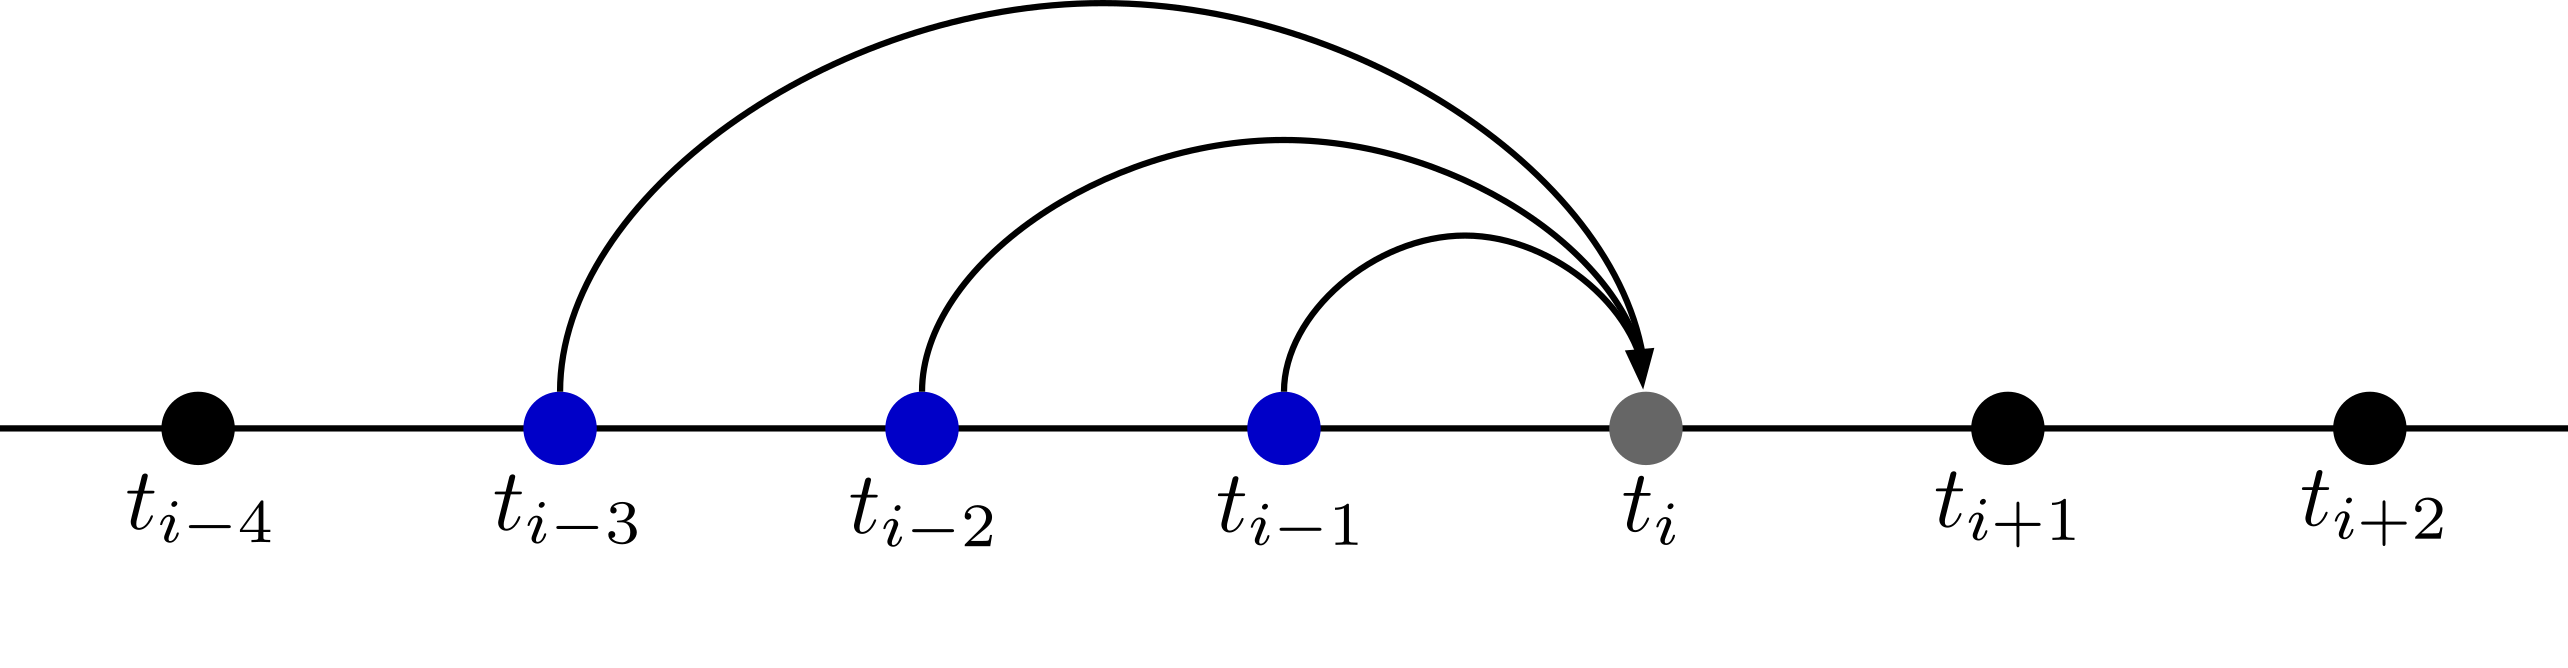
\includegraphics[scale=1]{images/higher_m.png}
  \caption{یک فرایند غیر مارکوف که حافظه‌ای به اندازه سه گام قبلی خود دارد}
\end{figure}
\FloatBarrier

\subsection{طول مارکوف}
اصولا تشخیص مارکوف بودن یا نبودن یک فرایند از روی داده‌های واقعی کار مشکلی است و دلیل اصلی آن این است که معمولا خاصیت مارکوف 
در فاصله‌های زمانی کوچک برقرار نیست. طول مارکوف به کوچک‌ترین مقیاسی گفته 
می‌شود که می‌توان یک فرایند تصادفی را مارکوف در نظر گرفت. یک فرایند تصادفی می‌تواند طول مارکوف متناهی یا نامتناهی داشته باشد.\cite{friedrich_approaching_2011} 
اگر بتوانیم چنین طولی را برای یک فرایند تصادفی پیدا کنیم می‌توانیم با استفاده از معادلات به دست آمده برای فرایندهای مارکوف دینامیک سیستم 
را با توجه به طول مارکوف بررسی کنیم. به عنوان مثال با توجه به رابطه ممان‌های شرطی با ضرایب بسط کرامرز-مویال یعنی رابطه 
\ref{cond_moment_km}، در صورتی که فرایند تصادفی مارکوف باشد رابطه آن با $\tau$ خطی است. و برای فرایندهای غیرمارکوف 
در صورتی که بتوانیم یک طول مارکوف به دست بیاوریم این رابطه خطی به ازای $\tau > l_m$ دیده می‌شود. 
در شکل زیر ممان‌های شرطی اول و دوم میدان سرعت برای یک سیال بر حسب $\Delta r$ رسم شده است. 
باید توجه داشته باشیم که در این مساله خاصیت مارکوف نسبت به $r$ سنجیده شده است. همانطور که می‌بینیم این ممان‌ها 
در این شکل خط چین عمودی نشان دهنده طول مارکوف $l_m$ است.
به ازای $\Delta r > l_m$ رفتار خطی با $\Delta r$ دارند.\cite{siefert2006joint}
\begin{figure}[H]
  \centering
  \subcaptionbox{}
  {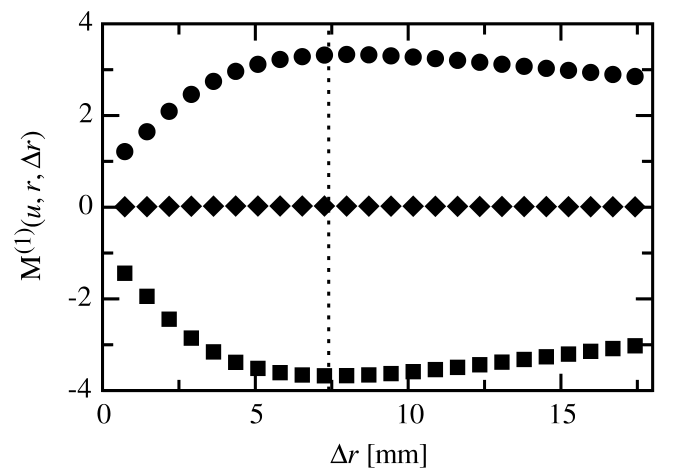
\includegraphics[width=0.49\textwidth]{images/fmoment.png}}
  \subcaptionbox{}
  {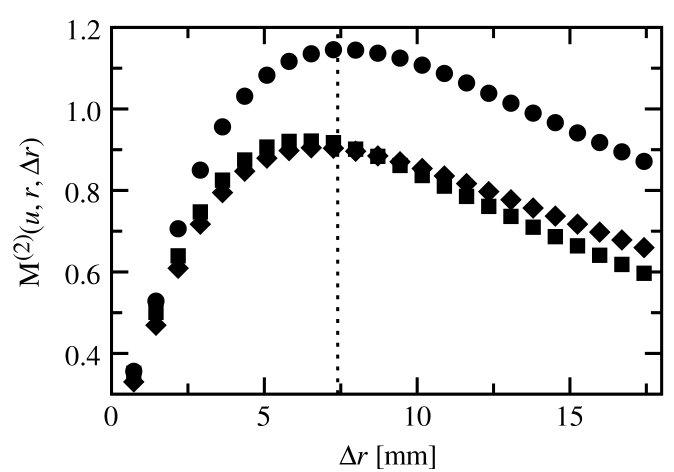
\includegraphics[width=0.49\textwidth]{images/smoment.png}}
  \caption{ممان‌های شرطی اول و دوم در میدان سرعت یک سیال برحسب مقیاس $\Delta r$، خط چین عمودی طول مارکوف را نشان می‌دهد.\cite{siefert2006joint}}
\end{figure}
\FloatBarrier

\section{تخمین طول مارکوف}
تا کنون سه روش برای محاسبه طول مارکوف ($l_m$) معرفی شده است که در این بخش این سه روش یعنی روش 
$\chi^2$، روش ویلکاکسون\LTRfootnote{Wilcoxon test} و آزمون چپمن-کولموگروف را توضیح خواهیم داد.

\subsection{روش $\chi^2$}

ایده اصلی در این روش مقایسه احتمال توأم سه نقطه‌ای یک فرایند با فرض مارکوف بودن و بدون فرض مارکوف بودن است. به عبارت دیگر احتمال توأم سه نقطه‌ای به شکل کلی زیر را در نظر بگیرید.
\begin{equation}
  p\left(x_{3}, t_{3} ; x_{2}, t_{2} ; x_{1}, t_{1}\right) = p\left(x_{3}, t_{3} | x_{2}, t_{2} ; x_{1}, t_{1}\right) p\left(x_{2}, t_{2} ; x_{1}, t_{1}\right)
\end{equation}
حال اگر فرض کنیم فرایند $x$ مارکوف است احتمال توأم سه نقطه‌ای آن را با $p_m$ نشان می‌دهیم و به شکل زیر در به دست می‌آید.
\begin{equation}
  p_{m}\left(x_{3}, t_{3} ; x_{2}, t_{2} ; x_{1}, t_{1}\right) = p\left(x_{3}, t_{3} | x_{2}, t_{2} \right) p\left(x_{2}, t_{2} ; x_{1}, t_{1}\right)
\end{equation}
اگر $x$ خاصیت مارکوف را داشته باشد این احتمال‌های توأم باید با هم برابر باشند، برای مقایسه این دو توزیع احتمال توأم از روش $\chi^2$ استفاده می‌کنیم. کمیت $\chi ^2$ را در نظر بگیرید که به شکل زیر تعریف می‌شود.
\begin{equation}
  \chi^{2} = \int d x_{3} d x_{2} d x_{1} \frac{\left[p\left(x_{3}, t_{3} ; x_{2}, t_{2} ; x_{1}, t_{1}\right) - p_{m}\left(x_{3}, t_{3} ; x_{2}, t_{2} ; x_{1}, t_{1}\right)\right]^{2}}{\left(\sigma_{3 j}^{2}+\sigma_{m}^{2}\right)}
\end{equation}
که $\sigma_{3 j}^{2}$ و $\sigma_{m}^{2}$ به ترتیب واریانس $p\left(x_{3}, t_{3} ; x_{2}, t_{2} ; x_{1}, t_{1}\right)$ و $p_{m}\left(x_{3}, t_{3} ; x_{2}, t_{2} ; x_{1}, t_{1}\right)$ هستند. برای تخمین $t_m$ از برآورد درست نمایی بیشینه استفاده می‌کنیم که به شکل زیر به دست می‌آید.

\begin{equation}
  \resizebox{1\hsize}{!}{$p\left(t_{3}-t_{1}\right) = \Pi_{x_{3}, x_{2} x_{1}} \frac{1}{\sqrt{2 \pi\left(\sigma_{3 j}^{2}+\sigma_{m}^{2}\right)}} \exp \left\{ - \frac{\left[p\left(x_{3}, t_{3} ; x_{2}, t_{2} ; x_{1}, t_{1}\right)-p_{m}\left(x_{3}, t_{3} ; x_{2}, t_{2} ; x_{1}, t_{1}\right)\right]^{2}}{2\left(\sigma_{3 j}^{2}+\sigma_{m}^{2}\right)}\right\}$}
\end{equation}
مشخص است برای آن که $p(t_3 - t_1)$ بیشینه باشد، $\chi^{2}_{\nu}$ باید کمینه بشود که $\chi_{\nu}^{2}=\frac{\chi^{2}}{N}$ و $N$ تعداد درجات آزادی است. بنابراین جایی که $\chi_{\nu}^{2}$ کمینه بشود معادل طول ماروکوف $t_m = t_3 - t_1$ است.\cite{kimiagar_markov_2011, ghasemi_markov_2007,kimiagar_markov_2008,friedrich_note_1998}
\begin{figure}[H]
    \centering
    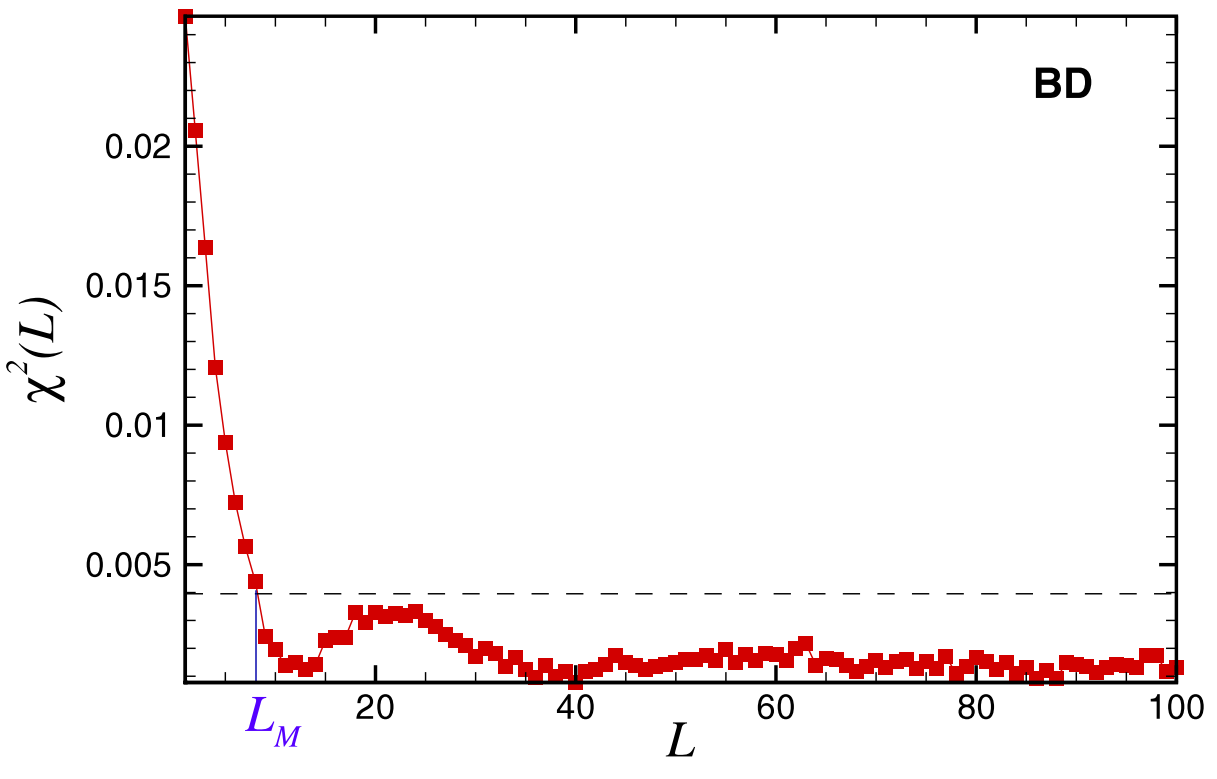
\includegraphics[width=0.9\textwidth]{images/x_v.png}
    \caption{معیار $\chi^{2}_\nu$ که طول مارکوف مدل \lr{Ballistic deposition} را نشان می‌دهد.\cite{kimiagar_markov_2008}}
  \end{figure}
  \FloatBarrier

\subsection{روش ویلکاکسون}

فرایند تصادفی $y$ و $z$ را در نظر بگیرید که از روی فرایند $x$ ساخته می‌شوند، به این شکل که فرایند $y$ نشان‌دهنده $x_{3}$  در زمان $t_{3}$ به این شرط که در زمان $t_{2}$، $x_{2}$ دیده شده باشد. فرایند $z$ نیز نشان‌دهنده $x_{3}$ در $t_{3}$ به شرطی که $x_{2}$ در $t_{2}$ و $x_{1}$ در $t_{1}$ مشاهده شده باشند، به عبارت دیگر داریم.
\begin{equation}
\begin{aligned} y\left(x_{2}, t_{3}, t_{2}\right) &=\left.x_{3}\left(t_{3}\right)\right|_{x_{2}\left(t_{2}\right)} \\ z\left(x_{2}, x_{1}, t_{1}, t_{2}, t_{3}\right) &=\left.x_{3}\left(t_{3}\right)\right|_{x_{2}\left(t_{2}\right), x_{1}\left(t_{1}\right)} \end{aligned}
\end{equation}
حال اگر $p(y) = \tilde{p}(z)$ باشد می‌گوییم فرایند مارکوف است، اما این دو چگالی احتمال هر دو نامشخص هستند. برای مقایسه این دو چگالی احتمال فرض کنید که نمونه‌های مستقل $y_{1}, \dotsc ,y_{n}$ و $z_{1}, \dotsc ,z_{m} y_{n}$ را از فرایندهای $y$ و $z$ داریم. حال اگر این داده‌ها را به شکل صعودی مرتب کنیم داریم.
\begin{equation}
y_{1}<y_{2}<z_{1}<y_{3}<z_{2}<z_{3}<y_{4}<\cdots
\end{equation}
برای بررسی فرض $p(y) = \tilde{p}(z)$ از تعداد وارونگی استفاده می‌کنیم، به تعداد $y_{j}$هایی که $y_{j} < z_{i}$ تعداد وارونگی $z_{i}$ گفته می‌شود. به عنوان مثال در نمونه بالا تعداد وارونگی‌های $z_{1}$ برابر ۲ است و تعداد وارونگی‌های $z_{2}$ برابر ۳ است. تعداد کل وارونگی‌ها برای تمام $z$ها را با $Q$ نمایش می‌دهیم. حال اگر $p(y) = \tilde{p}(z)$ باشد، $Q$ توزیع گاوسی دارد که میانگین آن برابر است با
\begin{equation}
\langle Q\rangle_{p=\tilde{p}}=\frac{m n}{2}
\label{exp_value_q}
\end{equation}
و واریانس $Q$ به ازای $n, m > 25$ برابر است با
\begin{equation}
  \sigma(m, n)^{2}=\frac{n m(n+m+1)}{12}
  \label{var_q}
\end{equation}
انحراف از مقدار چشم‌داشتی \ref{exp_value_q} معمولاً با قدر مطلق اختلاف $Q - \langle Q\rangle_{p=\tilde{p}}$ بررسی می‌شود.
\begin{equation}
  q=| Q-\langle Q\rangle_{p=\tilde{p}} | =q\left(x_{2}, x_{1}, t_{1}, t_{2}, t_{3}\right)
\end{equation}
فرض $p(y) = \tilde{p}(z)$ زمانی پذیرفته است که مقدار $q$ از یک کران مشخص کوچکتر باشد، این کران با استفاده از  یک به اصطلاح سطح اهمیت $\alpha$ مشخص می‌شود و معمولاً با $q_{\alpha}$ نمایش داده می‌شود. برای یک $\alpha$ مشخص، $q_{\alpha}$ به شکلی تعیین می‌شود که احتمال اینکه $q$ مقداری بزرگ‌تر از $q_{\alpha}$ داشته باشد برابر $\alpha$ بشود. به عبارت دیگر حتی اگر $p(y) = \tilde{p}(z)$ برقرار باشد هنوز هم به اندازه $\alpha$ این احتمال وجود دارد که $q$ مقداری بزرگ‌تر از $q_{\alpha}$ داشته باشد.
از آنجایی که $q$ قدر مطلق یک متغیر تصادفی با توزیع گاوسی با واریانس به شکل \ref{var_q} است، کران $q_{\alpha}$ را می‌توان با استفاده از معکوس تابع خطای گاوسی به دست آورد.\cite{waechter_stochastic_2004, wilcoxon_individual_1945, renner_experimental_2001, tutkun2004markovian}

\subsection{آزمون چپمن-کولموگروف}

روش سوم که برای تخمین طول مارکوف معرفی خواهد شد به طور مستقیم از معادله چپمن-کولموگروف استفاده خواهد کرد.
همان‌طور که قبلاً گفته شد معادله چپمن-کولموگروف \ref{ck_equation} برای فرایندهای مارکوف حتماً برقرار است، اما اگر این معادله برای فرایندی برقرار باشد این فرایند لزوماً مارکوف نیست. بنابراین 
برقرار بودن معادله چپمن-کولموگروف شرط لازم برای یک فرایند مارکوف است.
فرض کنید فرایند $x$ غیرمارکوف است. بنابراین معادله چپمن-کولموگروف به شکلی که برای 
یک فرایندهای مارکوف برقرار است برای فرایند $x$ برقرار نیست. اما اگر 
دو نقطه $x_i$ و $x_j$ که نشان دهنده 
فرایند تصادفی در زمان $t_i$ و $t_j$ هستند را در نظر بگیریم. می‌توانیم برقرار بودن یا نبودن 
معادله چپمن-کولموگروف را برای این نقاط بررسی کنیم. برای این کار نیاز است که $x_k$ که نشان‌دهنده 
فرایند تصادفی در $t_k$ که بین $t_i$ و $t_j$ است را در نظر بگیریم.
می‌توان با تعریف کمیت $S$ که نشان دهنده اختلاف دو طرف معادله چپمن-کولموگروف است برقرار بودن این معادله را ببینیم.
\begin{equation}
  S ( x_i, t_i; x_j, t_j ) =  p(x_{i},t_{i};x_{j},t_{j} ) - \int_{-\infty}^{+\infty} \mathrm{d} x_k p(x_{i},t_{i}|x_k,t_k) p(x_k,t_k;x_{j},t_{j})
  \label{chapmann_test}
\end{equation}
در واقع اگر رابطه چپمن-کولموگروف برای $x_i$ و $x_j$ برقرار باشد مقدار $S$ برابر با صفر خواهد بود و 
اگر این رابطه برقرار نباشد مقدار $S$ مخالف صفر است.
برای اینکه بتوانیم معیاری از آزمون چپمن-کولموگروف به ازای همه مقادیر به دست 
آوریم می‌توان از رابطه بالا قدرمطلق گرفت و سپس از آن نسبت به $x_i$ و $x_j$ انتگرال گرفت.
\begin{equation}
  S ( t_i, t_j ) = \int dx_i dx_j \left| S ( x_i, t_i; x_j, t_j ) \right|
  \label{chapmann_test_int}
\end{equation}
% \begin{equation}
%   \mathbf{S}_{i j} = \sum_{ij} \left| \mathbf{p}_{i j} - \mathbf{p}_{i k} \times \mathbf{p}_{k j} \right|
%   \label{chapmann_test}
% \end{equation} 
اگر در زمان‌های مشخص $t_{i}$ و $t_{j}$ که $t_{i} > t_{j}$، به ازای 
همه مقادیر $x_{i}$ و $x_{j}$ مقدار $S( x_i, t_i; x_j, t_j )$ برابر با 
صفر باشد، $S( t_i, t_j )$ 
نیز صفر می‌شود. بنابراین طول مارکوف $l_m = t_{i} - t_{j}$ است. ذکر این نکته لازم است که $S$ 
به ازای همه زمان‌های $t_k$ با این شرط که $t_{i} > t_k > t_{j}$ باید صفر باشد.\cite{fazeli_probing_2008}

اگر فرایند مورد نظر یک فرایند مانا باشد یا آن را مانا فرض کنیم می‌توان به جای محاسبه $S$ برای همه 
مقادیر $t_{i}$ و $t_{j}$ آن را بر حسب $\tau = t_{i} - t_{j}$ محاسبه کرد. 
برای جمله دوم رابطه \ref{chapmann_test} نیز می‌توانیم $\tau' = t_i - t_k$ و $\tau'' = t_k - t_j$ 
را در نظر بگیریم. بنابراین داریم:
\begin{equation}
  S ( x_i, x_j; \tau ) = p (x_{i},x_{j}; \tau ) - \int_{-\infty}^{+\infty} \mathrm{d} x_k p(x_{i}|x_k;\tau') p(x_k, x_{j};\tau'')
  \label{chapmann_test)stationary}
\end{equation}
و معادل رابطه \ref{chapmann_test_int} هم برای فرایند مانا می‌توانیم بنویسیم:
\begin{equation}
  S\left( \tau \right) = \int dx_i dx_j \left| S ( x_i, x_j; \tau ) \right|
  \label{chapmann_test_int_stationary}
\end{equation}
در شرایط عملی که ممکن 
است فقط یک سری زمانی داشته باشیم استفاده از رابطه \ref{chapmann_test_int} برای تخمین 
طول مارکوف ممکن نیست و باید از رابطه بالا استفاده کنیم.
%  برای اینکه $S$ را به ازای همه مقادیر $x_{i}$ و $x_{j}$ بررسی کنیم کمیت $S^{\prime}$ را به شکل زیر تعریف می‌کنیم
% \begin{equation}
%   S^{\prime}_{i j} = \int_{-\infty}^{+\infty} \int_{-\infty}^{+\infty} \mathrm{d} x_{i} \mathrm{d} x_{j}\left|S\left(x_{i}, x_{j}\right)\right|
%   \label{chapmann_test2}
% \end{equation}
% رفتار $S^{\prime}$ نسبت به $\Delta t = t_{j} - t_{i}$ مشابه $S$ است و از این پس برای تعیین طول مارکوف به روش آزمون چپمن-کولموگروف از کمیت $S^{\prime}$ استفاده می‌کنیم.
ذکر این نکته لازم است که، در شرایط عملی باید خطای محاسبه $S$ را نیز به دست بیاوریم و در نظر داشته 
باشیم که طول مارکوف در جایی تعیین می‌شود که $S$ با در نظر گرفتن خطا صفر خواهد شد.\cite{friedrich_approaching_2011}

در مسائلی که زمان گسسته است باید دقت کنیم که طول مارکوف برابر با $l_m=t_i - t_j - 1$ خواهد بود 
به این دلیل که همانطور که دیدیم معادله چپمن-کولموگروف برای یک فرایند مارکوف وقتی برقرار است 
که $\tau=2$ است اما طول مارکوف $l_m=1$ است. 
نکته مهم دیگر درباره این 
روش این است که $S$ را به ازای $\tau = t_i - t_j \leq 1$ نمی‌توان محاسبه کرد، بنابراین اگر برای فرایندی $S$ به ازای 
$\tau = 2$ صفر شد تنها می‌توان نتیجه گرفت که طول مارکوف این فرایند کوچک‌تر از $1$ است یعنی این فرایند یا مارکوف است یا مستقل از حالت‌های گذشته است.

\subsubsection{محاسبه خطا برای آزمون چپمن-کولموگروف}
برای محاسبه خطای $S$ می‌توان از مفهوم انتشار خطا استفاده کرد. در این روش با استفاده از خطای متغیرهای یک تابع می‌توان خطای تابع را 
محاسبه کرد. بدین منظور اگر $f(x_1,x_2,x_3, \cdots ,x_n)$ یک تابع با متغیرهای $x_1,x_2,
\cdots ,x_n$ باشد، می‌توان با رابطه زیر خطای $f$ را محاسبه کرد.
\begin{equation}
  \sigma_{f}=\sqrt{\left(\frac{\partial f}{\partial x_1}\right)^{2} \sigma_{x_1}^{2}+\left(\frac{\partial f}{\partial x_2}\right)^{2} \sigma_{x_2}^{2}+ \cdots + \left(\frac{\partial f}{\partial x_n}\right)^{2} \sigma_{x_n}^{2}}
  \label{error_propagation}
  \end{equation}
در رابطه بالا $\sigma_f$ نشان دهنده خطای $f$ و $\sigma_{x_1}, \sigma_{x_2}, \cdots , \sigma{x_n}$ نشان دهنده خطای متغیرهای $x_1, x_2, \cdots, x_n$ است.

بنابراین برای محسابه خطای $S$ ابتدا باید خطای توزیع‌های احتمال را به دست آورد. خطای یک توزیع احتمال یا توزیع احتمال شرطی را می‌توان با استفاده از رابطه زیر به دست آورد.\cite{prinz_markov_2011}
\begin{equation}
  \sigma_{p(x)}=\frac{\sqrt{p(x)(1-p(x) \mathrm{d} x)}}{ n \mathrm{d} x}
\end{equation}
با استفاده از این دو رابطه و رابطه \ref{chapmann_test} می‌توان خطای $S$ را به شکل زیر به دست آورد.
\begin{equation}
  \sigma_\mathbf{S} = \sqrt{\sigma_{p_{i j}}^2 + \sigma_{p_{i k}}^2 \times p_{k j}^2 + p_{i k}^2 \times \sigma_{p_{j k}}^2}
\end{equation}


\section{فرایندهای غیرمارکوف وابسته}
دو فرایند تصادفی $x$ و $y$ را در نظر بگیرید که غیر از خودشان یه یکدیگر نیز وابسته‌اند که این وابستگی می‌تواند دارای حافظه نیز باشد. شکل زیر نمایشی از وابستگی این دو فرایند به خودشان و به یکدیگر است. به این معنی که گذشته هر یک 
از فرایندها نه تنها در آینده خودشان تاثیر گذار است بلکه بر آینده فرایند دیگر نیز اثر می‌گذارد.
\begin{figure}[H]
  \centering
  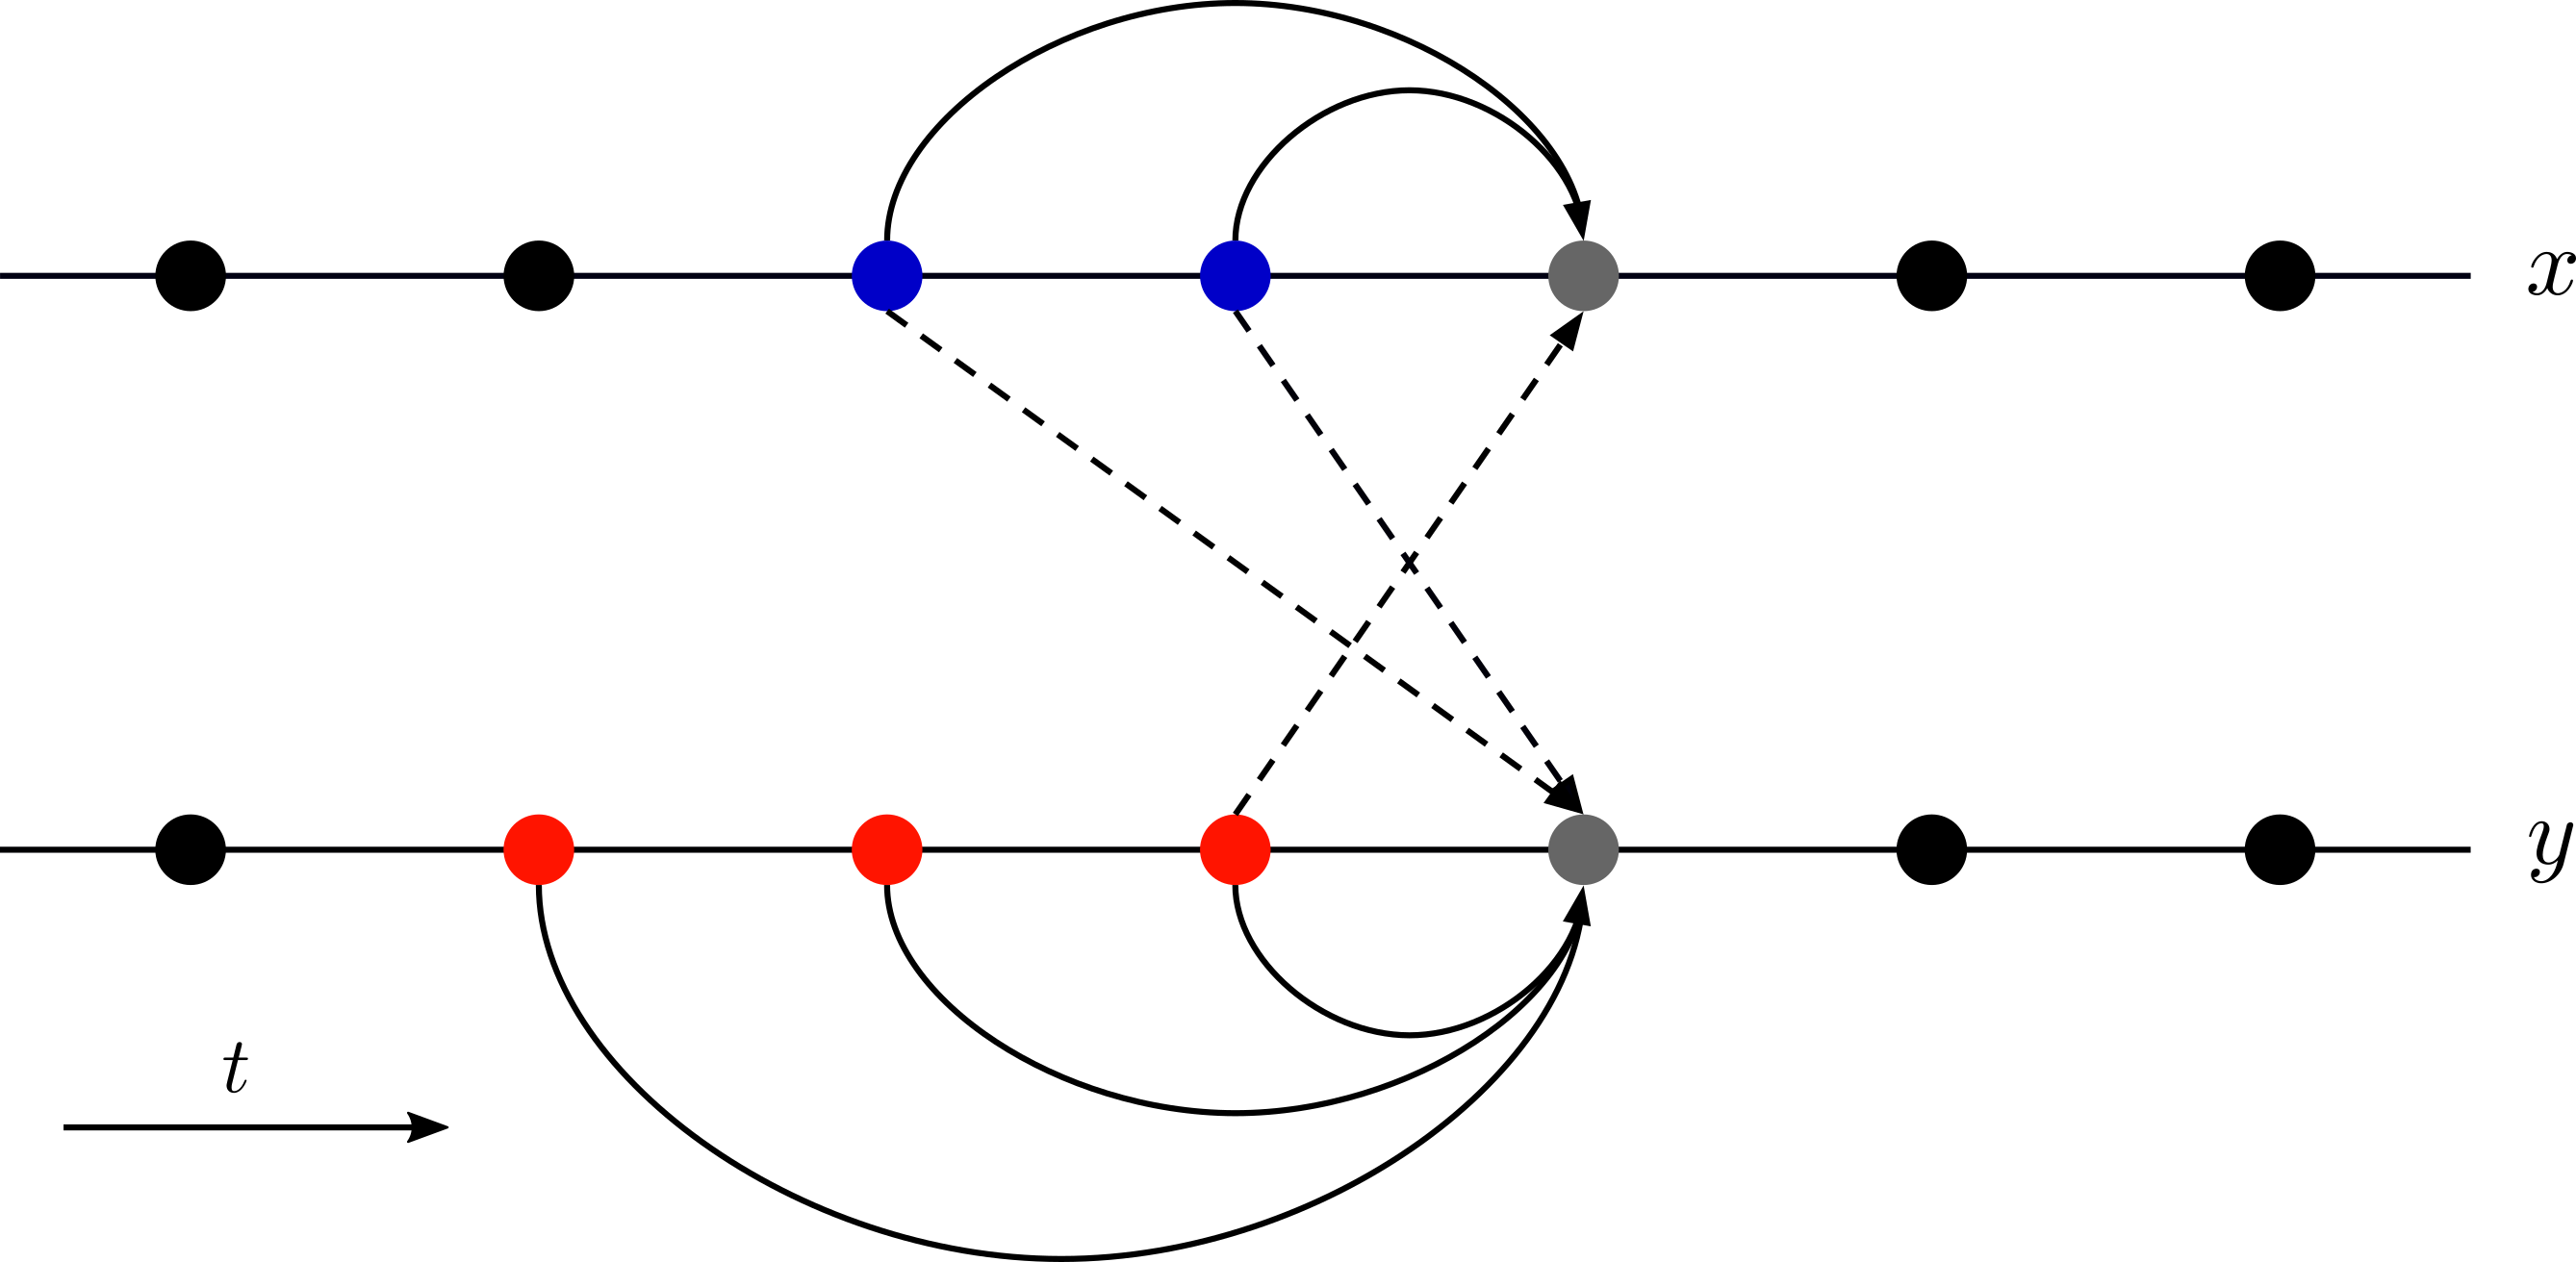
\includegraphics[scale=1]{images/coupled_hm.png}
  \caption{دو فرایند وابسته $x$ و $y$ که نسبت به یکدیگر و خودشان حافظه متفاوتی دارند. خطوط کامل حافظه نسبت به خود
  فرایند و خطوط خط چین حافظه نسبت به یکدیگر را نشان می‌دهند.}
\end{figure}
\FloatBarrier
می‌توان این دو فرایند را با استفاده از بردار تصادفی بررسی کرد. بردار $\vec{r}$ را به شکل زیر تعریف می‌کنیم.
\begin{equation}
  \vec{r} = (x, y)
  \label{stoch_vec}
\end{equation}
در این شرایط رابطه \ref{n_point_joint} را می‌توانیم به شکل زیر بازنویسی کنیم.
\begin{equation}
  \begin{array}{l}
  p(\vec{r}_n,t_n; \vec{r}_{n-1},t_{n-1} \dotsc ;\vec{r}_{0},t_0) \\ 
  \quad = p(\vec{r}_{n},t_n \mid \vec{r}_{n-1},t_{n-1} \dotsc ; \vec{r}_{0},t_{0}) \dotsc p(\vec{r}_{2},t_{2} \mid \vec{r}_{1},t_{1};\vec{r}_{0},t_{0}) p(\vec{r}_{1},t_{1} \mid \vec{r}_{0},t_{0}) p(\vec{r}_,t_0)
  \end{array}
  \label{n_point_joint_vec}
\end{equation}
ویژگی مارکوف برای این نوع فرایندها نیز قابل بررسی است. مشابه رابطه \ref{markov_def} فرایند برداری را مارکوف می‌گویند که رابطه زیر برای آن برقرار باشد.
\begin{equation}
  p(\vec{r}_n,t_n \mid \vec{r}_{n-1},t_{n-1} \dotsc ;\vec{r}_{0},t_0) = p(\vec{r}_n,t_n \mid \vec{r}_{n-1},t_{n-1})
  \label{markov_def_vec}
\end{equation}
و در نهایت برای توزیع احتمال توأم می‌توان نوشت.
 \begin{equation}
  \begin{array}{l}
    p(\vec{r}_n,t_n; \vec{r}_{n-1},t_{n-1} \dotsc ;\vec{r}_{0},t_0)\\ \qquad = p(\vec{r}_{n},t_n\mid \vec{r}_{n-1},t_{n-1}) \dotsc p(\vec{r}_{2},t_{2} \mid \vec{r}_{1},t_{1}) p(\vec{r}_{1},t_{1} \mid \vec{r}_{0},t_{0}) p(\vec{r}_0,t_0)
    \label{markov}
  \end{array}
\end{equation}
نکته قابل توجه و مهم در اینجا پیدا کردن طول مارکوف برای دو فرایند وابسته است که در این حالت فرایندهای $x$ و $y$ می‌توانند نسبت به خودشان و یکدیگر طول‌های متفاوتی داشته باشند. بدین منظور باید روش پیدا کردن طول مارکوف برای دو فرایند وابسته بازنویسی شوند. که در فصل آینده 
آزمون چپمن-کولموگروف را برای این فرایندها تعمیم خواهیم داد.

\section{مدل خودبرگشت}
برای آزمایش روش چپمن-کولموگروف برای تخمین طول مارکوف دو فرایند وابسته، در ابتدا بهتر است 
که در قدم اول با داده‌هایی کار کنیم که طول مارکوف آن‌ها را می‌دانیم. به این ترتیب می‌توان برخی از نقاط قوت
 و ضعف احتمالی را بهتر شناسایی کرد. برای این کار از مدلی به نام مدل خودبرگشت استفاده می‌کنیم.
یک مدل خودبرگشت از مرتبه $p$ که آن را با $AR(p)$ نشان می‌دهند به شکل زیر نوشته می‌شود.
\begin{equation}
  x_{t}=\sum_{n=1}^{p} \phi_n x_{t-n}+\xi_{t}
  \label{ar_model}
\end{equation}
ضرایب $\phi_n$ ضرایب ثابت غیر صفر هستند و $\xi_t$ یک نویز گاوسی با میانگین صفر و 
واریانس $\sigma_{\xi}^2$ است. میانگین $x_t$ در رابطه \ref{ar_model} برابر با صفر است 
اگر نیاز به ساخت سری زمانی با میانگین غیر صفر باشد کافی است $x_t$ با $x_t - \mu$ جایگزین 
بشود.\cite{shumway2011time}


 با رابطه بالا می‌توان سری‌های زمانی تولید کرد که به تعداد $p$ قدم به گذشته خودشان وابسته هستند. 
 در شکل \ref{fig:singleSample} یک نمونه از فرایند تصادفی رسم شده که 
 با رابطه \ref{ar_model} تولید شده است. برای تولید این سری زمانی مقادیر $p$ و $\phi_n$ به شکل زیر تعیین شده‌اند.
 $$
 p=18, \phi_n = \frac{0.3}{p}
 $$

 در صورتی که فقط یک نمونه با استفاده از رابطه \ref{ar_model} تولید کنیم، تنها قادر خواهیم بود که آزمون چپمن-کولموگروف 
را با فرض همگن بودن سری زمانی استفاده کنیم. در شکل \ref{fig:ToyModelSingleCK} نتیجه تست چپمن-کولموگروف را برای 
یک نمونه از فرایند \ref{ar_model} را می‌بینیم.
 \begin{figure}[H]
  \centering
  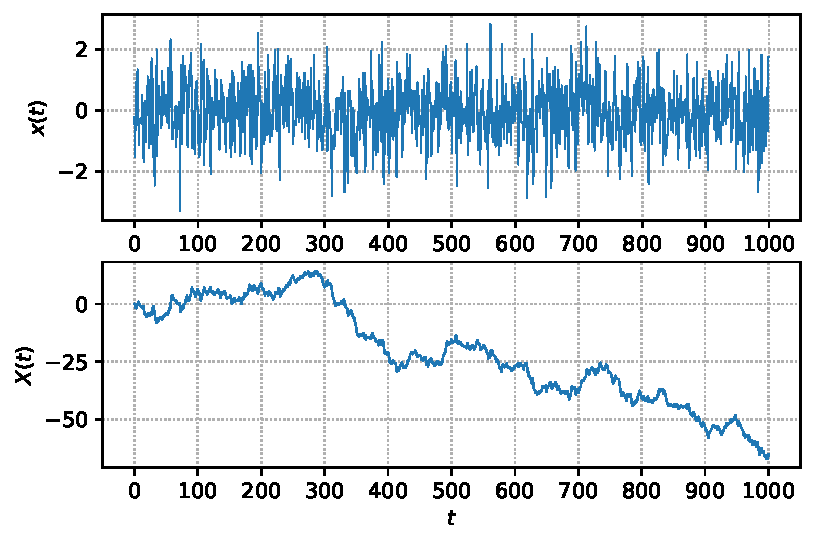
\includegraphics[width=\textwidth]{images/singleSample.pdf}
  \caption{یک نمونه از فرایند تصادفی که با استفاده از رابطه \ref{ar_model} با $p=18$ تولید شده است.\\ در این شکل $X_{t+1}=X_{t}+x_{t}$ است.}
  \label{fig:singleSample}
\end{figure}
% \FloatBarrier

\begin{figure}[H]
  \centering
  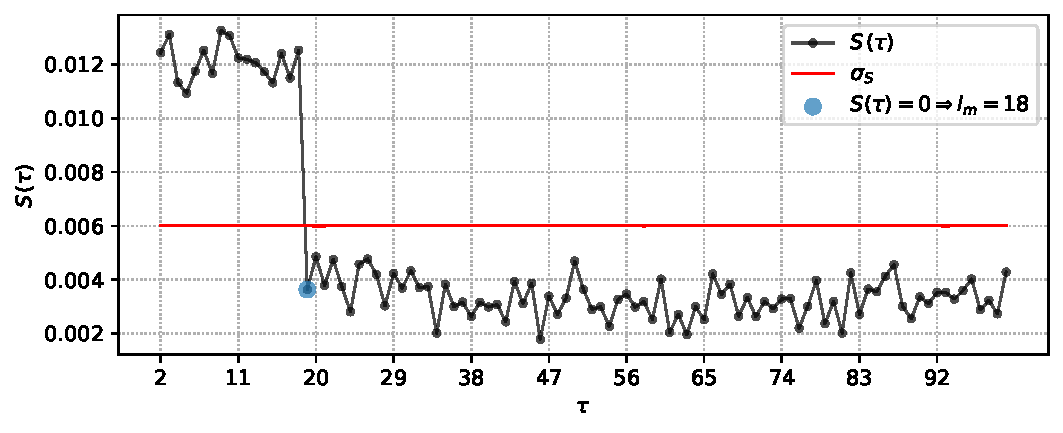
\includegraphics[width=\textwidth]{images/singleCKtestStat.pdf}
  \caption{آزمون چپمن-کولموگروف برای سری زمانی تولید شده با استفاده از \ref{ar_model}. مقدار $S(\tau)$ به ازای $\tau = 19$ با در نظر گرفتن خطا صفر شده است که نشان دهنده وابستگی فرایند $x$ به ۱۸ قدم قبلی خودش است.}
  \label{fig:ToyModelSingleCK}
\end{figure}
% \FloatBarrier
\begin{figure}[H]
    \centering
    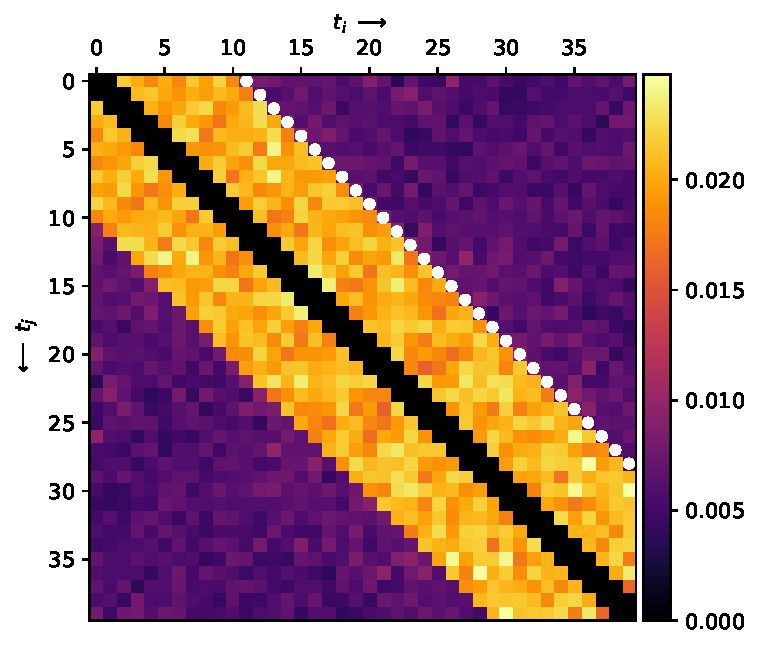
\includegraphics[width=0.8\textwidth]{images/singleCKtest.pdf}
    \caption{ماتریس $S(t_i,t_j)$ برای $3.5 \times 10^5$ نمونه با $p=10$.}
    \label{fig:ToyModelCK}
\end{figure}

همانطور که در شکل \ref{fig:ToyModelSingleCK} مشخص است مقدار $S(\tau)$ به ازای $\tau = 19$ با در نظر گرفتن خطا صفر شده‌است که نشان دهنده 
این مسأله است گه فرایند $x$ مستقل از حالت خود در ۱۹ قدم قبل است، اما به ۱۸ قدم قبلی خود وابسته است.

برای محاسبه ماتریس $S( t_i, t_j )$ به بیش از یک نمونه برای محاسبه توزیع‌های احتمال شرطی و توأم نیاز داریم. 
در شکل \ref{fig:ToyModelCK} نتیجه تست چپمن-کولموگروف برروی $3.5 \times 10^5$ نمونه رسم شده است. در این نمونه‌ها $p$ برابر با ۱۰ در 
نظر گرفته شده بود. در شکل \ref{fig:ToyModelCK} نقاط سفید نشان دهنده اوین جایی است که $S( t_i, t_j )$ با در نظر گرفتن 
خطا صفر شده است، همان طور که پیدا است به ازای $t_i - t_j = 11$ مقدار $S( t_i, t_j )$ با در نظر گرفتن خطا صفر شده است. 
که نشان دهنده تخمین درست $p = 10$ است.
